%%%%%%%%%%%%%%%%%%%%%%%%%%%%%%%%%%%%%%%%%%%%%%%%%%%%%%%%%%%%%%%%%%%%%%%%%%%%%%%%
%2345678901234567890123456789012345678901234567890123456789012345678901234567890
%        1         2         3         4         5         6         7         8

\documentclass[letterpaper, 10 pt, conference]{ieeeconf}  % Comment this line out if you need a4paper

%\documentclass[a4paper, 10pt, conference]{ieeeconf}      % Use this line for a4 paper

\IEEEoverridecommandlockouts                              % This command is only needed if 
                                                          % you want to use the \thanks command

\overrideIEEEmargins                                      % Needed to meet printer requirements.

% See the \addtolength command later in the file to balance the column lengths
% on the last page of the document

% The following packages can be found on http:\\www.ctan.org
%\usepackage{graphicx}
\usepackage{graphics} % for pdf, bitmapped graphics files
\usepackage{epsfig} % for postscript graphics files
\usepackage{subcaption}
\usepackage[noadjust]{cite}
%\usepackage{mathptmx} % assumes new font selection scheme installed
%\usepackage{times} % assumes new font selection scheme installed
\usepackage{amsmath,amssymb,amsfonts} % assumes amsmath package installed
%\usepackage{booktabs}

% format for theorems etc.
\newtheorem{thm}{\bfseries Theorem}
\newtheorem{lem}{\bfseries Lemma}
\newtheorem{cor}{\bfseries Corollary}
\newtheorem{prop}{\bfseries Proposition}
\newtheorem{rem}{\bfseries Remark}

% format for argmin, argmax
\newcommand{\argmax}{\operatornamewithlimits{argmax}}

% format for cross-reference
\usepackage[capitalize]{cleveref}
\crefname{equation}{eq.}{eq.}
\Crefname{equation}{Eq.}{Eq.}
\crefname{thm}{theorem}{theorems}
\Crefname{thm}{Theorem}{Theorems}
\crefname{lem}{lemma}{lemmas}
\Crefname{lem}{Lemma}{Lemmas}
\crefname{cor}{corollary}{corollaries}
\Crefname{cor}{Corollary}{Corollaries}
\crefname{prop}{proposition}{propositions}
\Crefname{prop}{Proposition}{Propositions}
\crefname{rem}{remark}{remarks}
\Crefname{rem}{Remark}{Remarks}

%=====todonotes===== %
\usepackage{todonotes}
\usepackage{soul}
\definecolor{smoothgreen}{rgb}{0.7,1,0.7}
\sethlcolor{smoothgreen}

\newcommand{\todopara}[1]{\vspace{0px} %
	\todo[inline, color=black!10]{\textbf{[Paragraph:]} {#1}} %
}
\newcommand{\todonote}[1]{\vspace{0px} %
	\todo[inline, color=green!30]{\textbf{[Note:]} {#1}} %
}
\newcommand{\todoQ}[1]{\vspace{0px} %
	\todo[inline, color=orange!50]{\textbf{[Note:]} {#1}} %
}
\newcommand{\todohere}[1]{\hl{(\textbf{TODO:} #1)}}

\newcommand{\hidetodos}{
	\renewcommand{\todopara}[1]{}
	\renewcommand{\todonote}[1]{}
	\renewcommand{\todoQ}[1]{}
	\renewcommand{\todohere}[1]{}}


\title{\LARGE \bf
Distributed Bayesian Filters for Multi-Robot Network by Using Latest-In-and-Full-Out Exchange Strategy of Observations}


\author{Chang Liu$^{1}$, Shengbo Eben Li$^{2}$ and J. Karl Hedrick$^{3}$% <-this % stops a space
\thanks{*The first two authors, C. Liu and S. Li, have equally contributed to this research. This work is supported by the Embedded Humans: Provably Correct Decision Making for Networks of Humans and Unmanned Systems project, a MURI project funded by the Office of Naval Research.}% <-this % stops a space
\thanks{$^{1}$Chang Liu is with the Vehicle Dynamics \& Control Lab, Department of Mechanical Engineering, University of California, Berkeley, Berkeley, CA 94709, USA. Email: {\tt\small changliu@berkeley.edu}}%
\thanks{$^{2}$Shengbo Eben Li is with the Department of Automotive Engineering, Tsinghua University, Beijing, 100084, China. He is currently working at Department of Mechanical Engineering, University of California, Berkeley as a visiting scholar. Email: {\tt\small lisb04@gmail.com}}%
\thanks{$^{3}$J. Karl Hedrick is with the Vehicle Dynamics \& Control Lab, Department of Mechanical Engineering, University of California, Berkeley, Berkeley, CA 94709, USA. Email: {\tt\small khedrick@me.berkeley.edu}}%
}


\begin{document}



\maketitle
\thispagestyle{empty}
\pagestyle{empty}


%%%%%%%%%%%%%%%%%%%%%%%%%%%%%%%%%%%%%%%%%%%%%%%%%%%%%%%%%%%%%%%%%%%%%%%%%%%%%%%%
\begin{abstract}

This paper presents a local exchange strategy of observations, i.e., Latest-In-and-Full-Out (LIFO), for distributed Bayesian filters (DBF) in a multi-robot network.
% for target search and tracking.
Different from statistics dissemination approaches that transmit posterior distributions or likelihood functions, each robot under LIFO only receives the latest available measurements and then broadcasts full communication buffer to its neighborhood, which significantly reduces the transmission burden of each pair from the order of environmental size to that of robot number.
Under the condition of fixed and undirected topology, LIFO can guarantee non-intermittent dissemination of all observations over the network within finite time.
%, with each robot non-intermittently receiving observations of all others.
Two types of LIFO-based DBF algorithms are proposed to estimate individual posterior density function (PDF) for static and moving target, respectively. 
For the static target, each robot locally fuses the newly received observations while for the moving target, a triangular matrix of historical observations is stored and updated. 
%Upon obtaining the latest available observations of all robots, an iterative Bayesian filtering procedure is applied that alternates between prediction and updating steps. 
The consistency of LIFO-based DBF is proved that individual PDF of each robot converges to the true target position when the number of observations tends to infinity.
%the agreement between robots' estimated target position and the actual position.
The effectiveness of this method is demonstrated by simulations.
\todohere{find out what convergence is}
\end{abstract}


%%%%%%%%%%%%%%%%%%%%%%%%%%%%%%%%%%%%%%%%%%%%%%%%%%%%%%%%%%%%%%%%%%%%%%%%%%%%%%%%
\section{INTRODUCTION}

Distributed filtering that focuses on using a group of networked robots to collectively infer environment status has been used for various applications, such as intruder detection \cite{chamberland2007wireless}, pedestrian tracking \cite{wang2007wlan} and micro-environmental monitoring \cite{cao2008development}. 
Several techniques have been developed for distributed filtering.
For example, Olfati-Saber (2005) proposed a distributed Kalman filter (DKF) for estimating states of linear systems with Gaussian process and measurement noise \cite{2005distributed}.
Each DKF used low-pass and band-pass consensus filters for the average-censensus of weighted measurements and inverse-covariance matrices.
Madhavan et al. (2004) presented a distributed Extended Kalman Filter (DEKF) for outdoor localization and mapping.
DEKF was used to generate local maps by using pose estimates to combine elevation gradient and vision-based depth with environmental features.
Gu (2007) proposed a distributed particle filter for target tracking over sensor networks \cite{gu2007distributed}. 
Gaussian mixture model (GMM) was adopted to approximate the posterior distribution from weighted particles and the parameters of GMM was exchanged via average consensus filter.
As a generic filtering scheme for nonlinear systems and arbitrary noise distributions, distributed Bayesian filter (DBF) has received increasing interest during past years \cite{bandyopadhyay2014distributed,hlinka2013distributed}, which is the focus of this study.
%This study focuses on developing a distributed Bayesian filter (DBF) that is applicable for state estimation of general nonlinear systems and the proposed DBF is applied to search and tracking (SAT) of both static and moving targets.

The design of distributed filtering algorithms is closely related to communication topology of multi-robot network, which can be classified into two types: fusion center-based and neighborhood-based.
In fusion center (FC)-based approaches, each robot uses a local filter to convert its own measurement into estimation of environment status, which is then transmitted (possibly via multi-hopping) to a FC.
At each filtering cycle, fusion center calculates the global state estimate only after receiving latest local estimates of all robots \cite{zuo2006bandwidth,vemula2006target}.
% has been a common structure for distributed filtering, in which local information collected by robots is transmitted (possibly via multi-hopping) to the fusion center for forming global estimation \cite{zuo2006bandwidth,ribeiro2006bandwidth}. 
%FC-based DBF is efficient for estimation in that it can collectively utilize all robots' information and thus useful for applications that only require information at a single central unit, such as in environmental monitoring.
%However, FC-based DBF requires constant communication link between each robot and the center, which is challenging for applications of robots in vast or complex areas.
In neighborhood (NB)-based approaches, all robots execute local filters and only communication between neighboring agents is allowed.
NB-based methods have become popular in recent years since such approaches do not require routing protocols or global knowledge about the network and therefore are robust to changes in the network topology and to link failures.
%, and thus suitable for networks with mobile agents.
%Besides, filtering is locally conducted on each robot, which requires less computation power compared to that in the fusion center.

%instead of communicating with a fusion center, each robot only exchanges information with neighboring robots and forms local estimation of the environment state. 
%NB-based DBF is advantageous over FC-based DBF in that no central unit is required, thus suitable for applications in which maintaining communication link between robots and center is challenging, such as in disaster situations.
%Besides, state estimation is locally conducted on each robot, which requires less computation power compared to that in the fusion center.

So far, most studies on NB-based DBF have mainly focused on the so-called \textit{statistics dissemination} strategy that each robot actually exchanges statistics , including posterior distributions and likelihood functions, with neighboring robots for distributed estimation.
\todohere{concern: this categorization is based on Hlinka's survery. Will this cause trouble? Besides, the name statistics dissemination and measurement dissemination are also from this survey. Any issues?}
DBFs using statistics dissemination strategy can be categorized into two types: leader-based and consensus-based. \cref{sheng2005distributed,}
In leader-based DBFs, environment status is sequentially passed and updated along a path formed by active robots, called leaders.
Only leaders perform DBF based on its own measurement and received measurements from local neighbors.
%\todohere{mention leader-based and consensus-based. 2 examples for leader-based and 3 examples for consensus-based.}
For example, Sheng et al. (2005) proposed a multiple leader-based distributed particle filter (DPF) with Gaussian Mixer for target tracking \cite{sheng2005distributed}.
% to track multiple moving targets. 
DPFs were run on a set of leader agents in uncorrelated sensor cliques and the particles were approximated as GMMs, the parameters of which were then exchanged among leaders for global estimation.
%In \cite{ram2007stochastic}, a circular topology that each sensor could only communicate with a fixed neighboring sensor was deployed for parameter estimation of a spatial field. 
%State estimates were updated using by sensors when passed along the circular topology Each sensor generates  based on that of the previous sensor and its own observation and sequentially passes the estimate to its neighbor.
In consensus-based DBFs, all robots locally execute filters simultaneously and diffuse the statistics among neighbors.
Global agreement of statistics among robots is achieved by using consensus algorithms, as proposed in \cite{olfati2007consensus,ren2005consensus,jadbabaie2003coordination}.
% by which all robots exchange statistics and executes consensus algorithms with neighbors, as proposed in , for fusion of statistics.
For example, Saptarshi et al. (2014) presented a Bayesian consensus filter (BCF) that uses logarithmic opinion pool for fusing posterior distributions of the tracked target among neighboring robots \cite{bandyopadhyay2014distributed}. 
%The proposed BCF can incorporate non-Gaussian uncertainties and nonlinearity in target dynamic models and measurement models. 
Julian et al. (2012) proposed a consensus-based distributed particle filter (DPF) that uses linear average consensus approach for fusing posterior functions of environment status. \cite{julian2012distributed}.
%The DPF can work even when the network diameter, the maximum in/out degree, and the number of robots are unknown.

%There are other types of variants, for example, in \cite{ram2007stochastic}, a circular topology that each sensor can only communicate with a fixed neighboring sensor is deployed for parameter estimation of a spatial field. 
%Each sensor generates state estimate based on that of the previous sensor and its own observation and sequentially passes the estimate to its neighbor.
%who using the incremental Robbins-Monro gradient algorithm locally at each sensor.

Despite the popularity of statistics dissemination strategy for NB-based DBFs, exchanging statistics can consume high communication resources, which can be infeasible in vast area or complex environment.
% such as marine search, seismological rescue, etc. 
Because of this, measurement dissemination strategy has been developed for NB-based DBFs, by which raw or quantized observations are exchanged among robots.
%This study focuses on the strategy of exchanging observations in the neighborhood of each robot, called the \textit{measurement dissemination-based} strategy, for the purpose of achieving a consensus of the probability density function (PDF) of the tracked target.  
Some pioneering studies have been done on this topic.
For example, Coates et al. (2004) used adaptive encoding of observations to minimize communication overhead for tracking a maneuvering object \cite{coates2004distributed}.
Ribeiro et al. (2006) presented distributed estimation based on quantized (binary) observations along with error-variance limits for several pragmatic signal models.
In a recent work, Djuric et al. (2011) proposed a distributed particle filtering for target tracking.
At each time, all robots broadcast their measurements to other agents, therefore each robot has a complete set of measurements of other robots for estimating target states \cite{djuric2011non}. 
%At each time instant, a subset of robots that are in proximity of the tracked targets share their observations for target position estimation.
% to all the remaining agents and apply local particle filter for target tracking 
%Another example can be found in \cite{rosencrantz2002decentralized}, in which both observations and statistics were exchanged among sensors for distributed surveillance of the environment.
In aforementioned works, communication topology is assumed fully connected that each robot can broadcast observations to all other robots in single transmission step.

This paper proposes a Latest-In-and-Full-Out (LIFO) strategy for distributed Bayesian filters (DBF) for undirected and connected communication topology. 
Each robot only broadcasts observations to its neighbors and implements Bayesian filter locally after receiving observations transmitted from neighboring robots.
The main benefit of LIFO is the reduction of communication burden, with the transmission data volume scaling linearly with the robot number, while statistics dissemination-based strategies suffer from the data volume on the order of environmental size.
%In addition, LIFO spreads all robots' observations among the network via multi-hopping, ensuring each robot's access to all others' historical observations.
%After receiving observations from neighbors, each robot runs Bayesian filter locally for environment state estimation. 
The proposed LIFO-based DBF has following properties:
(1)	For an undirected and connected network with fixed topology, LIFO guarantees the global dissemination of all robots' observations among the network via multi-hopping, with each robot non-intermittently receiving (delayed) observations of all other robots via local communication.
(2)	The corresponding DBF ensures consistency of the estimation of states, which refers to the agreement between robots' estimates of target position and the true position of the target. 
Moreover, consistency implies the consensus of robots' target PDFs.
In this study, the consistency and consensus using LIFO-DBF is formally proved.

The rest of this paper is organized as follows: 
The problem of distributed Bayesian filtering is formulated in \cref{sec:prob_form}.
The LIFO-based DBF algorithm is described in \cref{sec:LIFO-dbf}, followed by the proof of consistency and consensus in \cref{sec:consist_proof}.
Simulation results are presented in \cref{sec:sim} and \cref{sec:conclu} concludes the paper.

\section{PROBLEM FORMULATION}\label{sec:prob_form}
Consider a network of $N$ robots in a bounded two-dimensional space $S$. 
Each robot is equipped with a binary sensor for environmental perception. Due to the limit of communication range, each robot can only exchange observations with its neighbors. 
The Bayesian filter is run locally on each robot based on its own and received observations. 

\subsection{Probabilistic Model of Binary Sensor}
The goal of distributed Bayesian filter is to estimate the true target position by using a network of binary sensors.
The binary sensor only gives two types of observation: $1$ if the target is detected, and $0$ if no target is detected. 
The observation of $i^\text{th}$ sensor at $k^\text{th}$ time step is denoted as $z^i_k$.
The likelihood function that the target is detected is:
\begin{equation}\label{eqn:bin_sensor1}
P(z^i_k=1|x^T_k;x^R_k)\in \left[0,1\right],\; x^T_k\in S
\end{equation}
where $x^T_k$ denotes the target positions; $x^R_k$ is the robot position.
%; $X^T$ represents the set of all possible target positions.
Correspondingly, the likelihood function that no target is detected is:
\begin{equation}\label{eqn:bin_sensor0}
P(z^i_k=0|x^T_k;x^R_k)=1-P(z^i_k=1|x^T_k;x^R_k)
\end{equation}

The combination of \Cref{eqn:bin_sensor1} and \Cref{eqn:bin_sensor0} becomes a binary sensor model parameterized by $x^T_k$ and $x^R_k$. 
For the purpose of simplicity, we will not explicitly write $x^R_k$ for the rest of the paper.
%, with which all observations are generated. 
The commonly used likelihood functions for binary sensor include Gaussian function \cite{bonnie2012modelling,liu2014framework} and step function \cite{djuric2008target}.

\begin{rem}
	Given the knowledge of current target position, current observation of each robot is conditionally independent from both its own past observations and those of other robots.
\end{rem}

\begin{rem} 
	This study is applicable for both homogeneous and heterogeneous binary sensors. 
	A homogeneous model can simplify the analysis of completeness, while the heterogeneous model is more close to real sensing characteristics.
	In addition, it also works for other types of sensors, such as laser scanners \cite{hahnel2003efficient} and cameras \cite{tisdale2009autonomous}.
\end{rem}
\subsection{Graphical model of communication topology}
The robot network is always assumed to be connected.
Under this assumption, consider an undirected and fixed graph $G=(V,E)$, where $V=\left\lbrace 1,\dots,N\right\rbrace $ represents the index set of robots and $E=V\times V$ denotes the edge set. 
The adjacency matrix $M=\left[ m_{i,j}\right] $ describes the communication topology of $G$:
\begin{equation*}
m_{ij}=\begin{cases}
1& \text{if}\;\left(i,j\right)\in E\\
0& \text{if}\;\left(i,j\right)\notin E
\end{cases},
\end{equation*} 
where $m_{ij}$ denotes the entity of adjacency matrix. 
The notation $m_{ij}=1$ indicates that a communication link exists between $i^\text{th}$ and $j^\text{th}$ robot and $m_{ij}=0$ indicates no communication between them.

The \textit{direct neighborhood} of $i^\text{th}$ robot is defined as $\mathcal{N}_i=\left\lbrace j|m_{ij}=1,\forall j\in\left\lbrace1,\dots,N \right\rbrace \right\rbrace $. 
All the robots in $\mathcal{N}_i$ can directly exchange information with $i^\text{th}$ robot. 
In addition to direct neighborhood, another set called \textit{available neighborhood} is defined as $\mathcal{Q}_i$, which contains indices of robots whose observations are received by the $i^\text{th}$ robot given a specific observation exchange algorithm. 
Note that in general $\mathcal{N}_i\subseteq\mathcal{Q}_i$, but when only single-hopping is allowed, $\mathcal{N}_i=\mathcal{Q}_i$. 
\cref{fig:com_topo} illustrates three types of typical topologies: circular \cite{ram2007stochastic}, serial \cite{bahceci2005serial}, and star \cite{sheng2005distributed}. 
All of them are undirected and connected topologies.

\begin{figure}%[thpb]
	\centering
	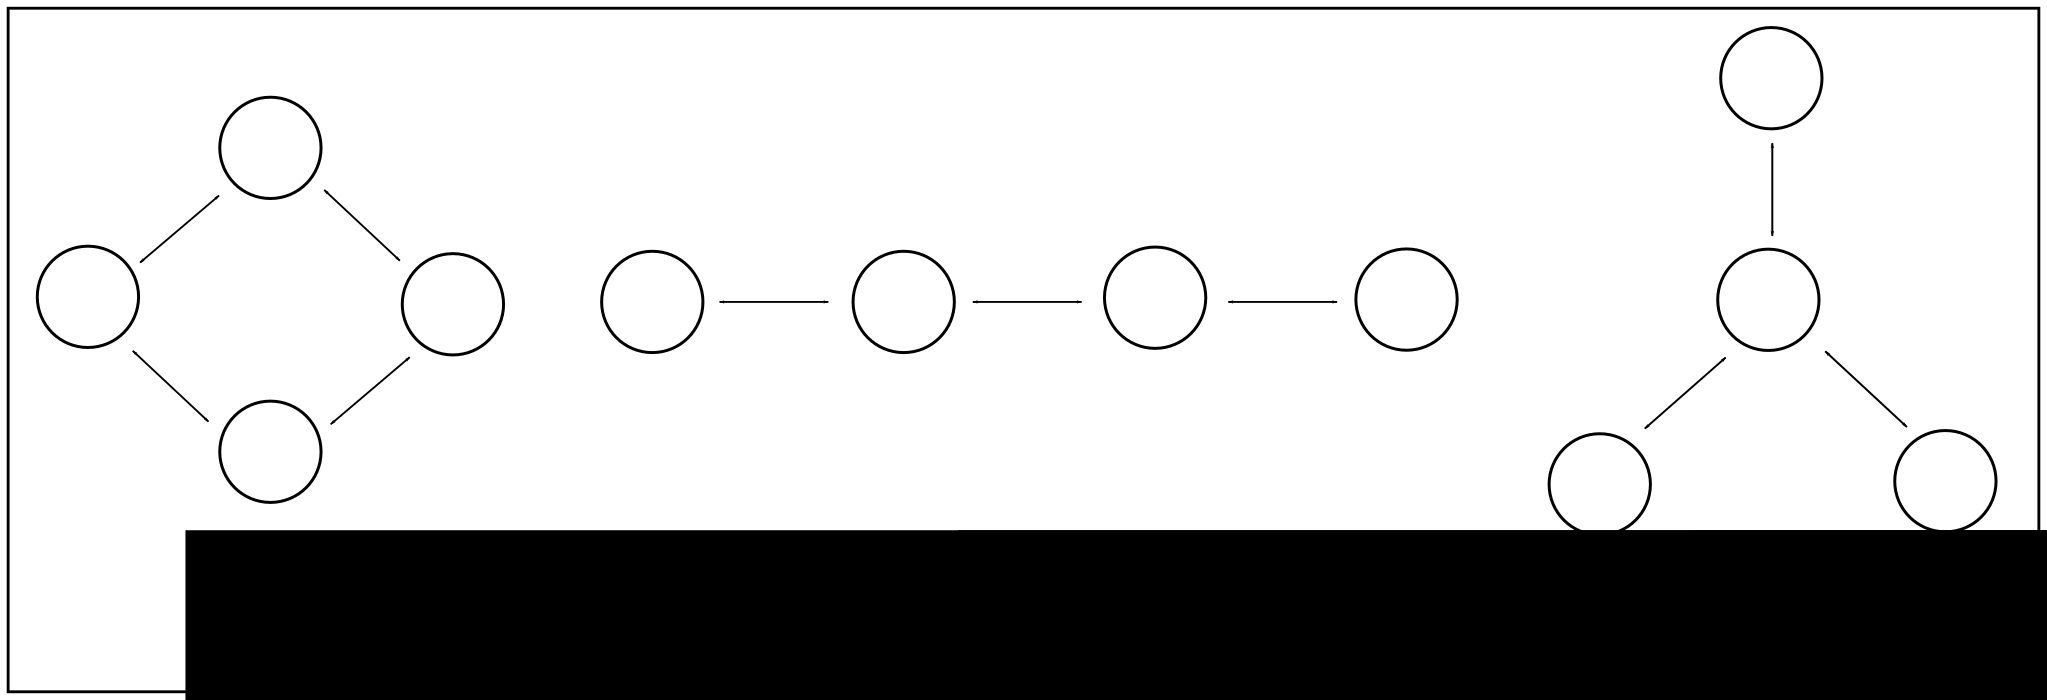
\includegraphics[width=0.45\textwidth]{figures/com_topo}
	\caption{Three types of topologies: (a)circular topology; (b)serial topology; (c)star topology}
	\label{fig:com_topo}
\end{figure}

\subsection{Distributed Bayesian Filter for Multiple Robots}\label{subsec:dbf}
The generic distributed Bayesian filter (DBF) is introduced in this section, which was also stated in \cite{hlinka2015distributed} and \cite{furukawa2006recursive}. 
Each robot has its individual estimation of posterior density function (PDF) of target position, called \textit{individual PDF}. 
The $i^\text{th}$ individual PDF at time $k$ is defined as $P^i_{pdf}(x^T_{k}|z^i_{1:k},z^{\mathcal{Q}_i}_{1:k})$. 
The individual PDF is initialized by the prior function $P^i_{pdf}(x^T_0|z^i_0,z^{\mathcal{Q}_i}_0)=P(x^T_0)$, given all available prior information including past experience and environmental knowledge. Under the framework of DBF, the individual PDF is recursively estimated by two steps, i.e., prediction step and updating step, based on the observations of $i^\text{th}$ robot and robots in $\mathcal{Q}_i$.
 
\subsubsection{Prediction}
%The $i^\text{th}$ individual PDF at time $k-1$ is known, denoted as $P^i_{pdf}(x^T_{k-1}|z^i_{1:k-1},z^{\mathcal{Q}_i}_{1:k-1})$. 
At time $k$, the prior individual PDF $P^i_{pdf}(x^T_{k-1}|z^i_{1:k-1},z^{\mathcal{Q}_i}_{1:k-1})$ is first predicted forward by using the Chapman-Kolmogorov equation:
\begin{align}\label{eqn:bayes_pred}
&P^i_{pdf}(x^T_k|z^i_{1:k-1},z^{\mathcal{Q}_i}_{1:k-1})\notag\\
&=\int P(x^T_k|x^T_{k-1})P^i_{pdf}(x^T_{k-1}|z^i_{1:k-1},z^{\mathcal{Q}_i}_{1:k-1})dx^T_{k-1}
\end{align}
where $P(x^T_k|x^T_{k-1})$ is a Markov motion model of the target, independent of robot states. 
This model describes the state transition probability of the target from a prior state $x^T_{k-1}$ to posterior state $x^T_k$. 
Note that the target is static in many search applications, such as the indoor search for stationary objects \cite{kulich2014single}. 
For a static target, its Markov motion model is simplified to be
\begin{equation*}
P(x^T_k|x^T_{k-1})=\begin{cases}
1 & \text{if}\; x^T_k=x^T_{k-1}\\
0 & \text{if}\; x^T_k\neq x^T_{k-1}
\end{cases}.
\end{equation*}
%and \Cref{eqn:bayes_pred} can be reduced to $P^i_{pdf}(x^T_{k}|z^i_{1:k-1},z^{\mathcal{Q}_i}_{1:k-1})=P^i_{pdf}(x^T_{k-1}|z^i_{1:k-1},z^{\mathcal{Q}_i}_{1:k-1})$.

\subsubsection{Updating}
At time $k$, the $i^\text{th}$ individual PDF is then updated by Bayes' formula using the latest available observations at time $k$: 
\small\begin{align}\label{eqn:bayes_upd}
&P^i_{pdf}(x^T_k|z^i_{1:k},z^{\mathcal{Q}_i}_{1:k})\notag\\
&=K_iP^i_{pdf}(x^T_k|z^i_{1:k-1},z^{\mathcal{Q}_i}_{1:k-1})P(z^i_k|x^T_k)\prod\limits_{j\in\mathcal{Q}_i}P(z^j_k|x^T_k)
\end{align}\normalsize
where $K_i$ is a normalization factor, given by:
\small\begin{align*}
K_i=1/\int P^i_{pdf}(x^T_k|z^i_{1:k-1},z^{\mathcal{Q}_i}_{1:k-1})P(z^i_k|x^T_k)\prod\limits_{j\in\mathcal{Q}_i}P(z^j_k|x^T_k)dx^T_k
\end{align*}\normalsize
where $P^i_{pdf}(x^T_k|z^i_{1:k},z^{\mathcal{Q}_i}_{1:k})$ is called posterior individual PDF; $P(z^i_k|x^T_k)$ is the likelihood function of observation $z^i_k$, described in \Cref{eqn:bin_sensor1} and \Cref{eqn:bin_sensor0}.

\section{Distributed Bayesian Filter via Local Exchange of Observations}\label{sec:LIFO-dbf}
This study proposes a Latest-In-and-Full-Out (LIFO) strategy for observation exchange and derives two corresponding distributed Bayesian filtering (DBF) algorithms, shorted as LIFO-DBF. 
The data communication in LIFO uses synchronized step as the execution of DBF.
In each step, LIFO only allows single-hopping communication within the neighborhood, but is able to broadcast observations of each robot to any other agents after a finite number of steps.
The individual PDF is forward predicted and updated in DBF after each LIFO cycle.
The theoretical analysis show that LIFO-DBF can ensure the consistency and consensus of distributed estimation while requiring much less communication burden than any statistics dissemination-based methods. 

\subsection{Strategy for Latest-In-and-Full-Out (LIFO)}\label{subsec:LIFO}
Under LIFO, each robot contains a communication buffer (CB) to store its latest knowledge of the observations of all robots: 
\begin{equation*}
\mathbf{z}^i_k=\left[ z^1_{k^i_1},\dots,z^N_{k^i_N}\right]
\end{equation*}
where $z^j_{k^i_j}$ represents the observation made by ${j^\text{th}}$ robot at time $k^i_j$. 
Note that under LIFO, $\mathcal{Q}_i=\left\lbrace 1,\dots,N\right\rbrace $, which will be proved in \Cref{cor1}.
At time k, $z^j_{k^i_j}$ is received and stored in ${i^\text{th}}$ robot CB, in which $k^i_j$ is the latest observation time of ${j^\text{th}}$ robot available to ${i^\text{th}}$ robot. Due to the communication delay, $k^i_j<k, \forall j\neq i$ always holds in practice.\\

The \textbf{LIFO strategy} is stated as follows:

%\begin{tabular}{l}
%\toprule
%LIFO Algorithm\\
%\midrule
(1) Initialization:
The buffer of $i^\text{th}$ robot is initialized when $k=0$: 
\begin{equation*}
%$\begin{array}{c}
	z^j_{k^i_j}=\emptyset,\; k^i_j=0,\;j=1:N
%\end{array}$\\
\end{equation*}

(2) At $k^\text{th}$ step for $i^\text{th}$ robot :

(2.1) Receiving Step:

The $i^\text{th}$ robot receives all CBs of its neighboring robots. 
The received CBs are totally $|\mathcal{N}_i|$ groups, each of which corresponding to the (k-1)-step CB of a robot in $\mathcal{N}_i$. 
The received CB from $l^\text{th}$ ($l\in \mathcal{N}_i$) robot is denoted as
\begin{equation*}
\mathbf{z}^l_{k-1}=\left[ z^1_{(k-1)^l_1},\dots,z^N_{(k-1)^l_N}\right],\; l\in\mathcal{N}_i
\end{equation*}

(2.2) Observation Step: 

The $i^\text{th}$ robot updates $z^j_{k^i_j}\,(j=i)$ by its own observation at current step:
\begin{equation*}
z^j_{k^i_j}=z^i_k,\;k^i_j=k,\;\text{if }j=i.
\end{equation*}

(2.3) Comparison Step:

The $i^\text{th}$ robot updates other elements of its own CB, i.e., $z^j_{k^i_j}\,(j\neq i)$, by selecting the latest information among all received CBs from $\mathcal{N}_i$. For all $j\neq i$,
\begin{align*}
l_\text{latest}&=\argmax_{l\in \mathcal{N}_i,i}\left\lbrace\left(k-1\right)^i_j,\left(k-1\right)^l_j  \right\rbrace\\
z^j_{k^i_j}&=z^j_{\left(k-1\right)^{l_\text{latest}}_j},\; k^i_j=\left(k-1\right)^{l_\text{latest}}_j
\end{align*} 

(2.4) Sending Step:

The $i^\text{th}$ robot broadcasts its updated CB to all of its neighbors defined in $\mathcal{N}_i$.
%\bottomrule
%\end{tabular}

\begin{figure}%[thpb]
	\centering
	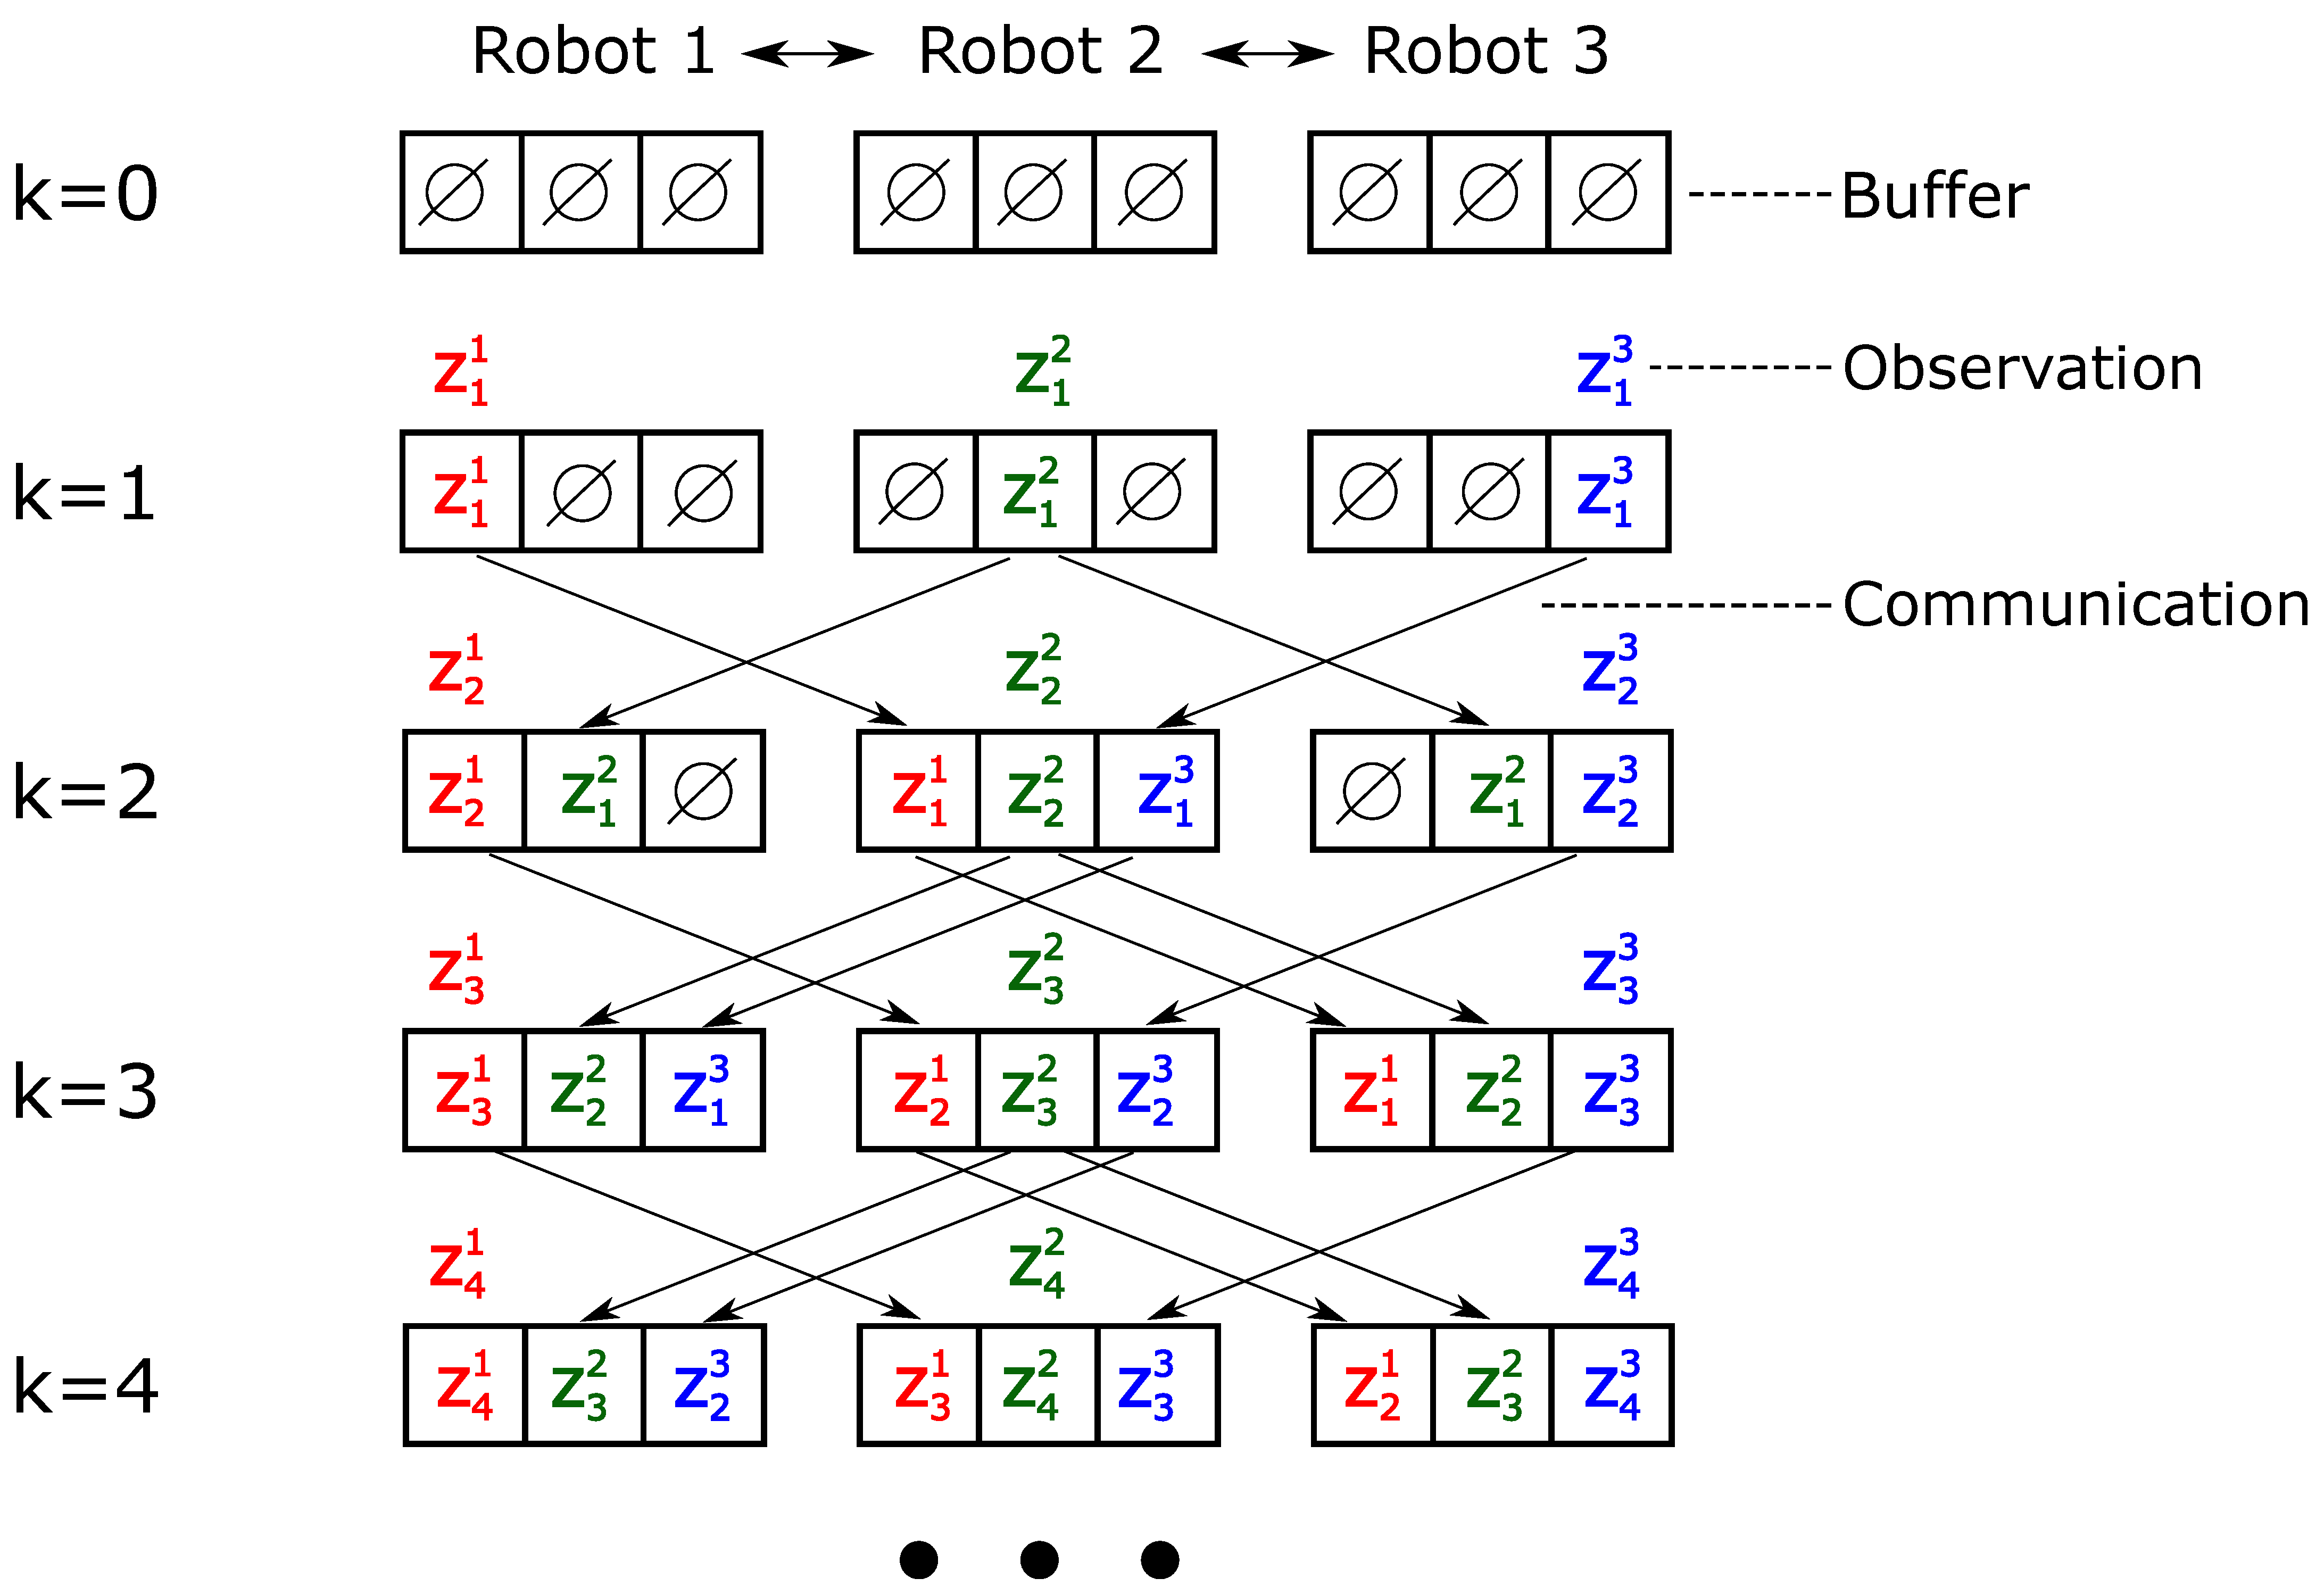
\includegraphics[width=0.48\textwidth]{figures/data_exchange}
	\caption{Example of LIFO with three robots using serial communication topology}
	\label{fig:LIFO}
\end{figure}
(3) $k\leftarrow k+1$ until stop $\hfill\blacksquare$\\

\cref{fig:LIFO} illustrates the LIFO cycles with 3 robots using a serial topology. 
Two facts can be noticed in \cref{fig:LIFO}: (1) all robot CBs are filled within 3 steps, which means under LIFO each robot has a maximum delay of 2 steps for receiving observations from other robots; (2) after filled, the updating of CBs are non-intermittent, which means each robot continuously receives new observations of other robots. Extending the two facts to a network of $N$ robots, we have the following proposition:
\medskip
\begin{prop}\label{prop1}
For a fixed and undirected network of $N$ robots, LIFO uses the shortest path(s) between $i^\text{th}$ and $j^\text{th}$ robot to exchange observation, the length of which equals the delay $\tau_{i,j}$ between them.
\end{prop}
\begin{proof} 
Without loss of generality, assume that there is a unique shortest path between $i$ and $j$, denoted by $T^{j,i}_{n^*}=\left(v_1,\dots,v_{n^*}\right)$, with $v_1=j,v_{n^*}=i,v_{m+1}\in\mathcal{N}_{v_m}$. 
Then, the distance between $i$ and $j$ is $d(j,i)=n^*-1$. 
The following mathematical induction will prove \Cref{prop1}.

Step (1): When $d(j,i)=1$, $j\in\mathcal{N}_i$ and $j$ can directly send $z^j_k$ to $i$. Then $z^j_k$ is stored in $i^\text{th}$ CB at time $k+1$, i.e. $\tau_{i,j}=1$. 
\Cref{prop1} holds for $d(j,i)=1,\;i,j\in\left\lbrace 1,\dots,N\right\rbrace $.

Step (2): Suppose that \Cref{prop1} holds for $d(j,i)=s,\;s\geq 2$. 
Then for $d(j,i)=s+1$, i.e., $n^*=s+2$, by the Bellman's principle of optimality, the path $T^{j,l}_{n^*-1}=\left(v_1,\dots,v_{n^*-1}\right)$ is a shortest path between $j$ and $l$, where $v_{n^*-1}=l$ and $i\in \mathcal{N}_l$. 
The assumption that \Cref{prop1} holds for $d(j,i)=s$ implies that $z^j_k$ is received and stored in $l^\text{th}$ robot's CB at time $k+s$. 
Since $i\in\mathcal{N}_i$, $i^\text{th}$ robot receives $z^j_k$ at $k+s+1$. 
For any other path $T^{j,i}_{n}=\left(v_1,\dots,v_{n}\right)$ with $n>n^*$, $z^j_k$ cannot be received by $i$ earlier than $k+s+1$. 
Therefore $\tau_{i,j}=s+1$. 
This proves the \Cref{prop1} for $d(j,i)=s+1$.
\end{proof}
%\vspace{\baselineskip}
\medskip
\begin{cor}\label{cor1}
For the same topology in \Cref{prop1}, all elements in $\mathbf{z}^i_k$ under LIFO become filled when $k\geq N$.	
\end{cor}
\begin{proof}
In a network of $N$ robots, the maximal length of shortest paths is no greater than $N-1$. Based on \Cref{prop1}, $\tau_{i,j}\leq N-1$ and thus all elements of $\mathbf{z}^i_k$ become filled when $k\geq N$.
\end{proof}
\medskip
\begin{cor}\label{cor2}
For the same topology in \Cref{prop1}, once all elements in $\mathbf{z}^i_k$ are filled, the updating of each element is non-intermittent. 	
\end{cor}
\begin{proof}
For a network with fixed topology, shortest path(s) between any nodes are fixed. 
Therefore, based on \Cref{prop1}, $\tau_{i,j}$ is constant and the updating of each element in $\mathbf{z}^i_k$ is non-intermittent.
\end{proof}
\medskip
\begin{rem}
	Compared to statistics dissemination, LIFO is more communication-efficient for distributed filtering. 
	To be specific, consider an $M\times M$ grid environment with a network of $N$ robots, the transmitted data of LIFO between each pair of robots are only the CB of each robot, the length of which is $O(N)$. 
	On the contrary, the length of transmitted data for a statistics dissemination approach is $O(M^2)$, which is the size of the environment. 
	Since $M$ is generally much larger than $N$ in target search and tracking, LIFO requires much less communication resources.
\end{rem}

\subsection{Algorithm of LIFO-DBF for Static Target}\label{subsec:LIFO-dbf-sta-tar} 

This section derives the LIFO-DBF algorithm for localizing a static target. 
Each robot stores last-step individual PDF, i.e., $P^i_{pdf}(x^T|\mathbf{z}^i_{1:k-1})$. 
The assumption of static target can simplify the Bayesian filter as the prediction step becomes unnecessary. 
Therefore, the $i^\text{th}$ individual PDF is only updated by 
\begin{equation}\label{eqn:LIFO-dbf-sta-tar}
P^i_{pdf}(x^T|\mathbf{z}^i_{1:k})=K_iP^i_{pdf}(x^T|\mathbf{z}^i_{1:k-1})\prod\limits_{j=1}^{N}P(z^j_{k^i_j}|x^T)
\end{equation}
where
\begin{equation*}
K_i=1/\int P^i_{pdf}(x^T|\mathbf{z}^i_{1:k-1})\prod\limits_{j=1}^{N}P(z^j_{k^i_j}|x^T)dx^T
\end{equation*}

\subsection{Algorithm of LIFO-DBF for Moving target}\label{subsec:LIFO-dbf-mov-tar}
This section derives the LIFO-DBF for localizing a moving target. 
Instead of storing last-step PDF, each robot maintains an individual PDF of time $(k-N)$ and a triangular matrix of historical observations from time $(k-N+1)$ to current time $k$. 
The $i^\text{th}$ individual PDF is then alternatively predicted and updated by using aforementioned Bayesian filter (\Cref{eqn:bayes_pred} and \Cref{eqn:bayes_upd}) from $(k-N)$ to $k$.
\cref{fig:LIFO-DBF} illustrates the LIFO-DBF procedure for the $1^\text{st}$ robot as an example.
\begin{figure}%[thpb]
	\centering
	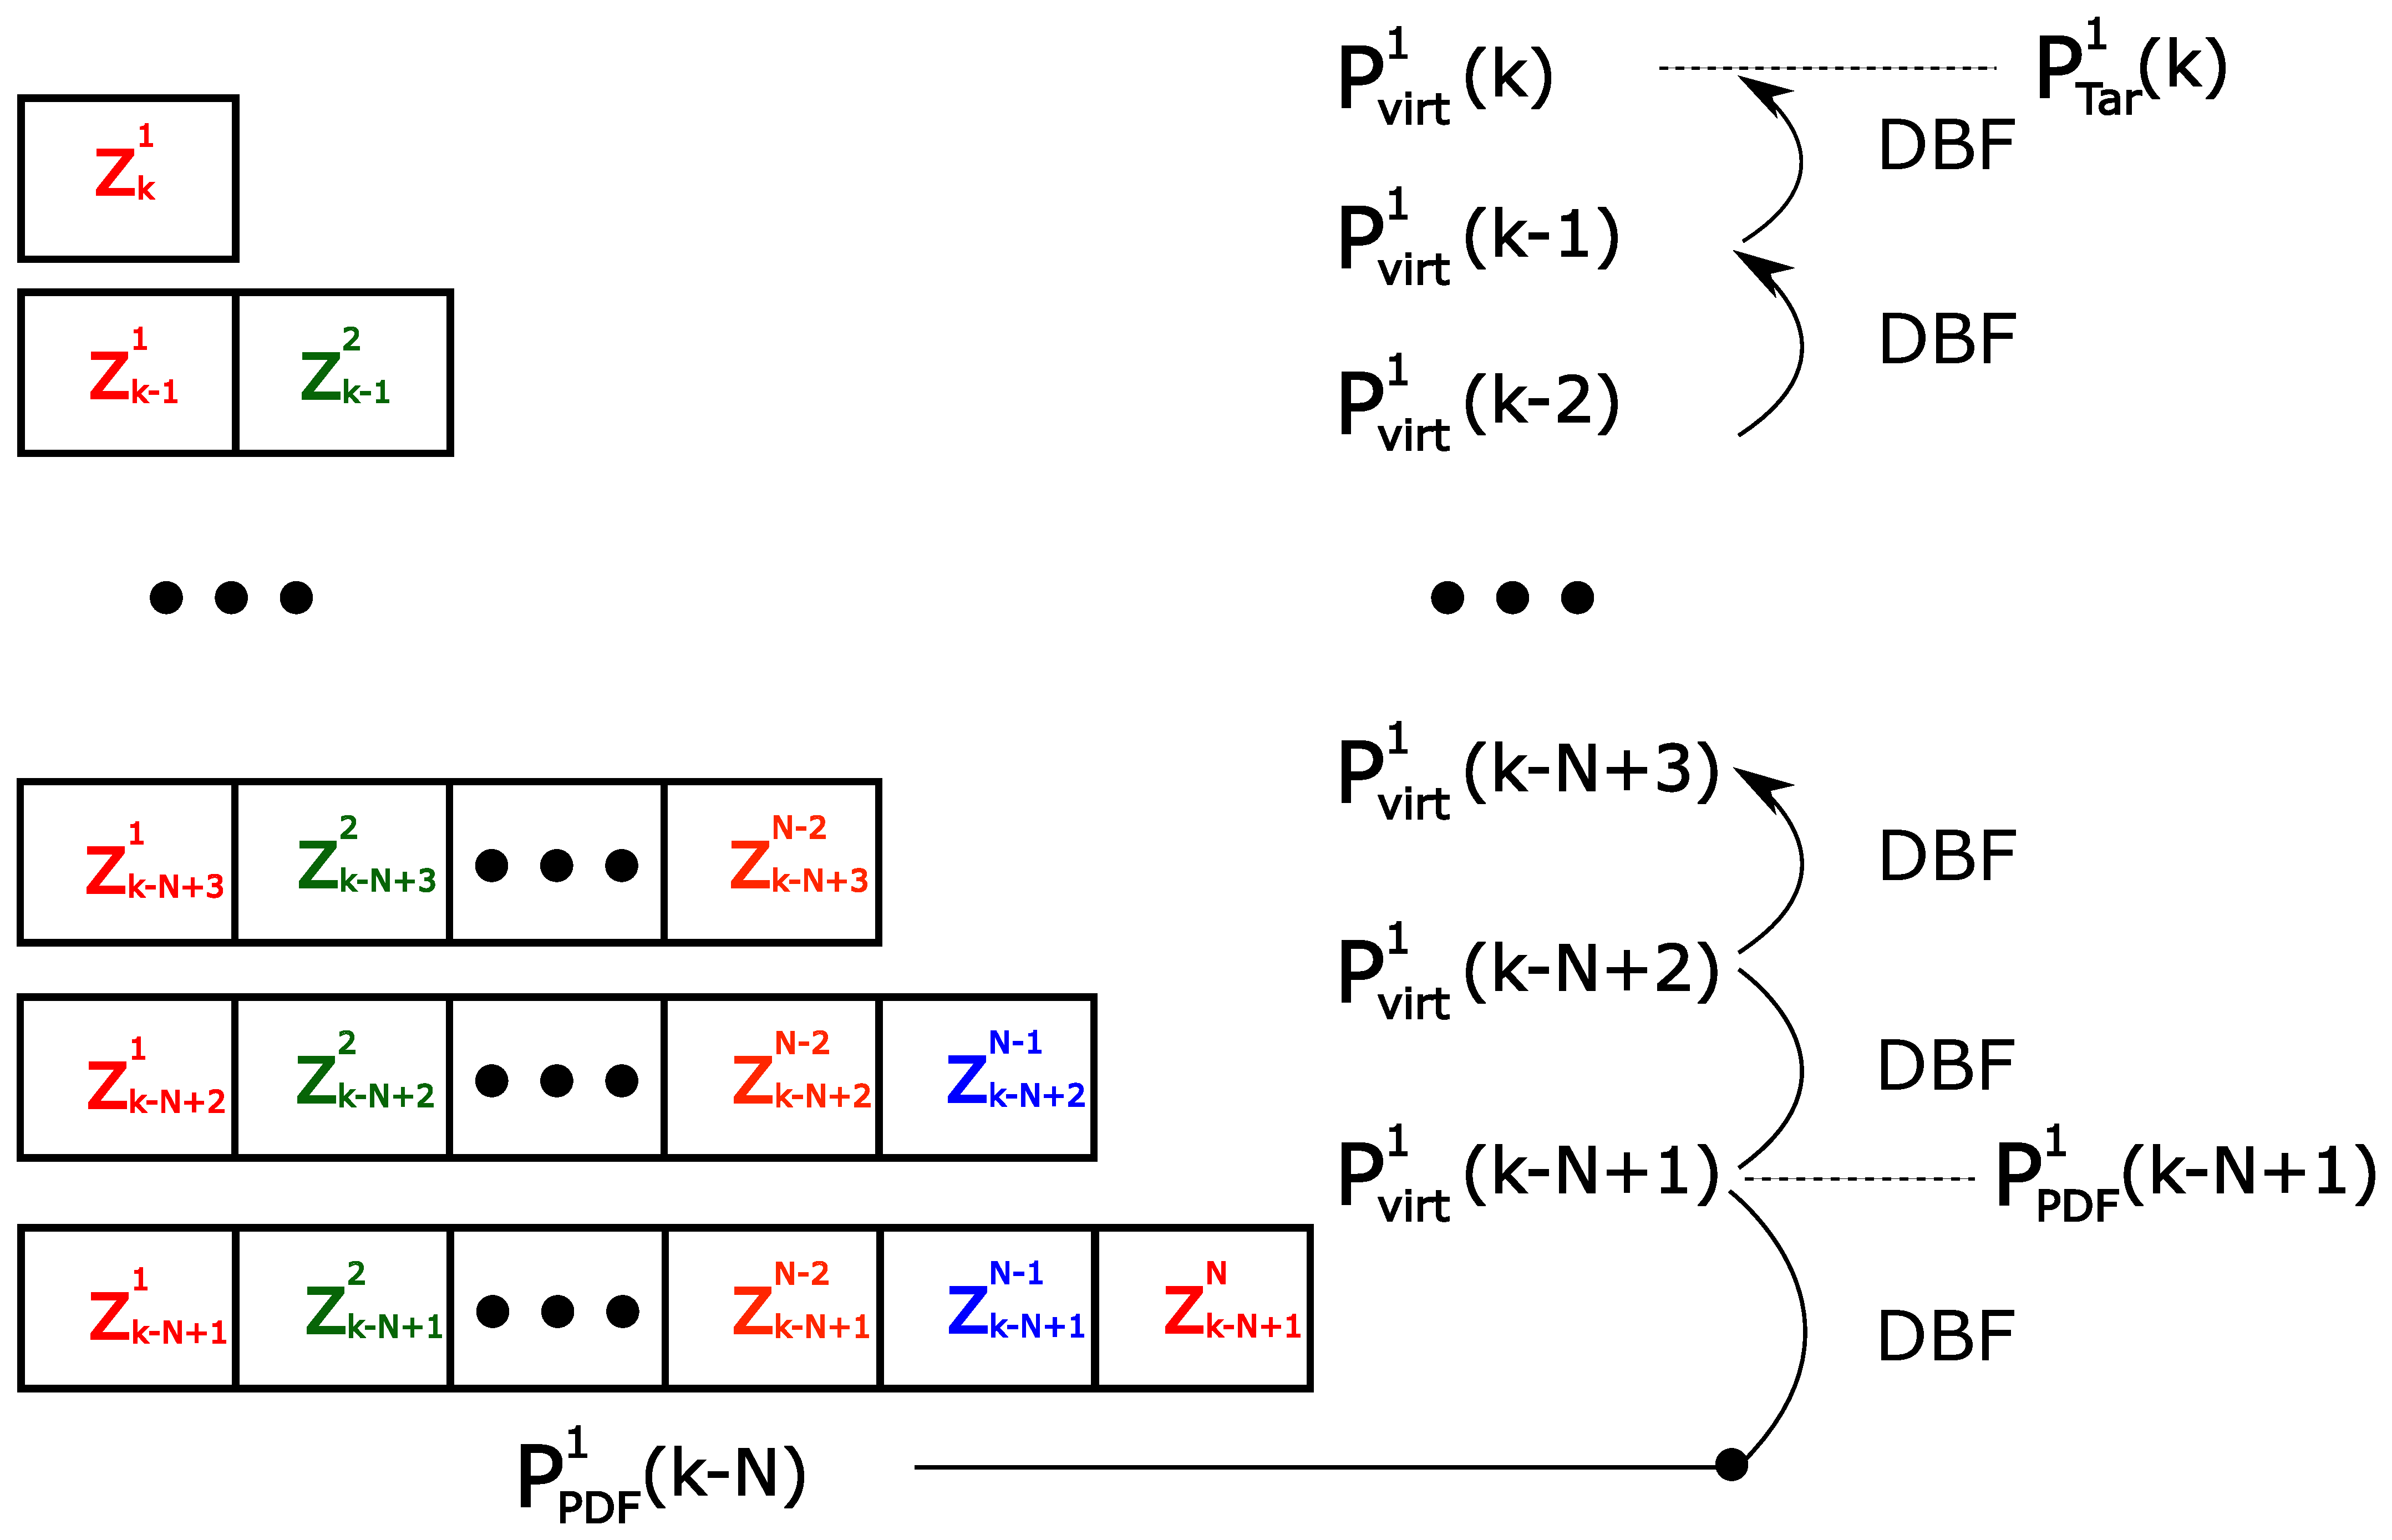
\includegraphics[width=0.47\textwidth]{figures/DBF_demo}
	\caption{Example of LIFO-DBF for $1^\text{st}$ robot at time $k$. The current individual PDF is $ P^1_{pdf}(x^T_{k-N}|z^1_{1:k-N},\dots,z^N_{1:k-N})$, denoted as $ P^1_{pdf}(k-N)$ in the figure. The robot first calculates $ P^1_{virt}(k-N+1)$ using DBF and stores it as $ P^1_{pdf}(k-N+1)$. Repeating DBF until obtaining $ P^1_{pdf}(k)$, which is then used as the target PDF estimation of $1^\text{st}$ robot at time $k$.}
	\label{fig:LIFO-DBF}
\end{figure}
The generic \textbf{LIFO-DBF algorithm} for moving target is stated as follows:
%\begin{enumerate}

For $i^\text{th}$ robot at $k^\text{th}$ step:

	\textbf{(1)} The stored individual PDF for time $(k-N)$ is:
	\small\begin{equation*}
		P^i_{pdf}(x^T_{k-N}|z^1_{1:k-N},\dots,z^N_{1:k-N})
	\end{equation*}\normalsize
	
	\textbf{(2)} Initialize a virtual PDF by assigning the individual PDF to it:
	\small\begin{equation*}
		P^i_{virt}(x^T_{k-N})=P^i_{pdf}(x^T_{k-N}|z^1_{1:k-N},\dots,z^N_{1:k-N})
	\end{equation*}\normalsize
		
	\textbf{(3)} From $\xi=1$ to $N$, repeat two steps of Bayesian filtering:
%	\begin{enumerate}
%		\item 

		(3.1) Prediction 
		\small\begin{align*}
		&P_{virt}^{pre}(x^T_{k-N+\xi})\\=&\int P(x^T_{k-N+\xi}|x^T_{k-N+\xi-1})P^i_{virt}(x^T_{k-N+\xi-1})dx^T_{k-N+\xi-1}
		\end{align*} \normalsize
				
%		\item 
		(3.2) Updating
		\small\begin{gather*}
		P^i_{virt}(x^T_{k-N+\xi})=K_\xi P_{virt}^{pre}(x^T_{k-N+\xi})\prod\limits_{j\in\Omega^i_{\xi}}P(z^j_{k-N+\xi}|x^T_{k-N+\xi})\\
		K_\xi=1/\int P_{virt}^{pre}(x^T_{k-N+\xi})\prod\limits_{j\in\Omega^i_{\xi}}P(z^j_{k-N+\xi}|x^T_{k-N+\xi})dx^T_{k-N+\xi}
		\end{gather*} \normalsize
%	\end{enumerate}
	
	\textbf{(4)} Store the first-step virtual PDF as the individual PDF for time $(k-N+1)$
	\begin{equation*}
		P^i_{pdf}(x^T_{k-N+1}|z^1_{1:k-N+1},\dots,z^N_{1:k-N+1})=P^i_{virt}(x^T_{k-N+1}).
	\end{equation*}
	$\hfill\blacksquare$
	
%\end{enumerate}

%1)	The stored individual PDF for $(k-N)^\text{th}$ step is $ P^i_{pdf}(x^T_{k-N}|z^1_{1:k-N},\dots,z^N_{1:k-N})$.
%
%2)	Initialize a virtual PDF by assigning the individual PDF to it:
%$P_{virt}(x^T_{k-N})=P^i_{pdf}(x^T_{k-N}|z^1_{1:k-N},\dots,z^N_{1:k-N})$
%
%3)	From $\xi=1$ to N, repeat two steps of Bayesian filtering
%(a)	Prediction 
%\begin{align*}
%&P_{virt}^{pre}(x^T_{k-N+\xi})\\=&\int P(x^T_{k-N+\xi}|x^T_{k-N+\xi-1})P_{virt}(x^T_{k-N+\xi-1})dx^T_{k-N+\xi-1}
%\end{align*} 
%(b)	Updating
%\begin{gather*}
%P_{virt}(x^T_{k-N+\xi})=K_\xi P_{virt}^{pre}(x^T_{k-N+\xi})\prod\limits_{j\in\Omega^i_{k-N+\xi}}P(z^j_{k_N+\xi|x^T_{k-N+\xi}})\\
%K_\xi=1/\int P_{virt}^{pre}(x^T_{k-N+\xi})\prod\limits_{j\in\Omega^i_{k-N+\xi}}P(z^j_{k-N+\xi}|x^T_{k-N+\xi})dx^T_{k-N+\xi}
%\end{gather*} 
%  
%4)	Store the first-step virtual PDF as the $(k-N+1)^\text{th}$ individual PDF: $P^i_{pdf}(x^T_{k-N+1}|z^1_{1:k-N+1},\dots,z^N_{1:k-N+1})=P_{virt}(x^T_{k-N+1}).$

Note that $\Omega^i_{\xi}$ denotes the index set of robots whose observation at time $(k-N+\xi)$ is stored in $i^\text{th}$ robot's CB. 
The individual PDF of $i^\text{th}$ robot at time $k$ is $P^i_{virt}(x^T_k)$.
\medskip
\begin{rem}
	For the static target, each robot only needs current step CB to update individual PDFs. 
	Therefore, except storing individual PDFs, all historical CBs can be discarded and only current-step CB is stored in robot memory, the length of which is $O(N)$. 
	On the contrary, for the moving target, each robot needs to store a triangular matrix of history observation (except current step CB) with size of $O(N^2)$ and an individual PDF with size $O(M^2)$, which means that the size of occupied memory in each robot is $O(M^2+N^2)$.
\end{rem}

\section{Proof of Consistency and Consensus}\label{sec:consist_proof}

This section proves consistency and consensus of LIFO-DBF. 
Only proofs for localizing static target using static robots and moving robots are presented.
The proof of LIFO-DBF for moving target is similar to that of static target by considering the dynamic model of the target, but with more complicated algebraic manipulation. 

Assume that $S$ is finite and $x^{T^*}$ is the true location. Define an \textit{equivalent-location} set $X^T_{eq}\subseteq S$ such that 
\small\begin{equation*}
X^T_{eq}=\left\lbrace x^T\in S|P(z_k|x^{T})=P(z_k|x^{T^*}),\; \forall z_k\in \left\lbrace 0,1\right\rbrace\right\rbrace ,
\end{equation*}\normalsize
i.e., $x^T$ gives the same the observation likelihood as $x^{T^*}$ for given robot positions.
%for any two parameters in $X^T_{eq}$, the sensor model with one of these two parameters generates equivalent probability value for the same observation $z_k$
Since $X^T$ is finite, $X^T_{eq}$ is also finite. 
%Let $X^T_{eq,1},\dots,X^T_{eq,u}$ denote all equi-parameter sets that partition $X^T$ such that following properties hold:
%\begin{enumerate}
%	\item $\bigcup^u_{i=1} X^T_{eq,i}= X^T$
%	\item $X^T_{eq,i}\cap X^T_{eq,j}=\emptyset,\;i,j\in \left\lbrace 1,\dots,u\right\rbrace ,i\neq j.$
%\end{enumerate}
%Without loss of generality, assume $x^{T^*}\in X^T_{eq,1}$, where $x^{T^*}$ denotes the actual position of the target. 

%\todohere{double check if the following examples for equi-parameter set are accurate}

%\begin{rem}
%	the equivalent-location set depends on the property of the sensor. 
%	For example, for a laser scanner with high-fidelity sensing capability, each equivalent-location set contains only a small number of target positions.
	The reason to introduce equivalent-location set is that ghost target might exist in some special robot arrangement and sensor types.
	For example, for undirected binary sensors that are linearly arranged, a ghost target can exist at the mirror position of the true target.
	When sensors are overlapped at a single point, ghost targets can exist on a circle that contains the true target.
	In theory, DBF cannot rule out ghost targets in such cases and prior knowledge is needed for further clarification.
	This study only proves the convergence to the equivalent-location set rather to the true location.
	
%\end{rem}

\subsection{Proof for static robots}
The consistency of LIFO-DBF for static robots is stated as follows: 
\begin{thm}\label{thm:LIFO-dbf-sta-tar}
	For static robots, each individual PDF converges to $ X^T_{eq}$ using LIFO-DBF when the number of observations tends to infinity, i.e.
	\begin{equation*}
	P^i_{pdf}(x^T\in X^T_{eq}|\mathbf{z}^i_{1:k})\longrightarrow
%	\begin{cases}
%	1 & \text{if}\; i=1\\
%	0 & \text{if}\; i\neq 1
%	\end{cases},\;
	1,\;
	k\rightarrow \infty
	\end{equation*}
	where $\mathbf{z}^i_{1:k}=\left(z^1_{1:k_1},\dots,z^N_{1:k_N}\right) $.
%	, $\left\lbrace k_1,\dots,k_N\right\rbrace $ are the timestamps of the $i^\text{th}$ robot's latest knowledge of all robots' observations.
\end{thm}

\begin{proof}	
Considering the conditional independence of observations $z^j_k$ for given $x^T\in S$, the batch form of DBF at $k^\text{th}$ step is:
\small\begin{subequations}
	\begin{align*}
		P^i_{pdf}(x^T|\mathbf{z}^i_{1:k})&=P^i_{pdf}(x^T|z^1_{1:k_1},\dots,z^N_{1:k_N})\\
		&=\frac{P^i_{pdf}(x^T)\prod\limits_{j=1}^{N}\prod\limits_{l=1}^{k_j}P(z^j_l|x^T)}{\sum\limits_{x^T\in S}\prod\limits_{j=1}^{N}\prod\limits_{l=1}^{k_j}P(z^j_l|x^T)},
	\end{align*}
\end{subequations}\normalsize
where $P^i_{pdf}$ is $i^\text{th}$ robot's initial individual PDF. 
It is known from \Cref{cor1} and \Cref{cor2} that $k-N<k_j\leq k$.
\addtocounter{equation}{-1}\\

Compare $P^i_{pdf}(x^T|\mathbf{z}^i_{1:k})$ with $P^i_{pdf}(x^{T^*}|\mathbf{z}^i_{1:k})$:
\small\begin{equation}\label{eqn:cmp}
\frac{P^i_{pdf}(x^T|\mathbf{z}^i_{1:k})}{P^i_{pdf}(x^{T^*}|\mathbf{z}^i_{1:k})}=\frac{P^i_{pdf}(x^T)\prod\limits_{j=1}^{N}\prod\limits_{l=1}^{k_j}P(z^j_l|x^T)}{P^i_{pdf}(x^{T^*})\prod\limits_{j=1}^{N}\prod\limits_{l=1}^{k_j}P(z^j_l|x^{T^*})}
\end{equation}\normalsize

Take the logarithm of \Cref{eqn:cmp} and average it over k steps:
\small\begin{equation}\label{eqn:cmp_log}
 \frac{1}{k}\ln\frac{P^i_{pdf}(x^T|\mathbf{z}^i_{1:k})}{P^i_{pdf}(x^{T^*}|\mathbf{z}^i_{1:k})}=\frac{1}{k}\ln\frac{P^i_{pdf}(x^T)}{P^i_{pdf}(x^{T^*})}+\sum\limits_{j=1}^{N}\frac{1}{k}\sum\limits_{l=1}^{k_j}\ln\frac{P(z^j_l|x^T)}{P(z^j_l|x^{T^*})}
\end{equation}\normalsize

Since $P^i_{pdf}(x^T)$ and $P^i_{pdf}(x^{T^*})$ are bounded,
\begin{equation}\label{eqn:cmp_lim1}
\lim\limits_{k\rightarrow \infty}\frac{1}{k}\ln\frac{P^i_{pdf}(x^T)}{P^i_{pdf}(x^{T^*})}\longrightarrow 0
\end{equation}

The binary observations subject to Bernoulli distribution $B(1,p_j)$, yielding
\begin{equation*}
P^i_{pdf}(z^j_k|x^T)=p^{z^j_k}_j(1-p_j)^{1-z^j_k}
\end{equation*}
where $p_j=P(z^j_k=1|x^T)$. Utilizing the facts: (1) $z^j_l$ are conditionally independent samples from $B(1,p_j^*)$ and (2) $k-N<k_j\leq k$, the law of large numbers yields
\begin{equation*}
\lim\limits_{k\rightarrow \infty}\frac{1}{k}\sum\limits_{l=1}^{k_j}z^j_l=p^*_j,\quad \lim\limits_{k\rightarrow \infty}\frac{1}{k}(k_j-\sum\limits_{l=1}^{k_j}z^j_l)=1-p^*_j
\end{equation*}
where $p_j^*=P(z^j_k=1|x^{T^*})$. Then, 
\small\begin{equation}\label{eqn:cmp_lim2}
\lim\limits_{k\rightarrow \infty}\frac{1}{k}\sum\limits_{l=1}^{k_j}\ln\frac{P(z^j_l|x^T)}{P(z^j_l|x^{T^*})}=p^*_j\ln \frac{p_j}{p^*_j}+(1-p^*_j)\ln \frac{1-p_j}{1-p^*_j}
\end{equation}\normalsize

Note that the right-hand side of \Cref{eqn:cmp_lim2} achieves maximum if and only if $p_j=p_j^*$. 
Considering \Cref{eqn:cmp_lim1} and \Cref{eqn:cmp_lim2}, the limit of \Cref{eqn:cmp_log} is:
\small \begin{equation}\label{eqn:lim}
 \lim\limits_{k\rightarrow \infty}\frac{1}{k}\ln\frac{P^i_{pdf}(x^T|\mathbf{z}^i_{1:k})}{P^i_{pdf}(x^{T^*}|\mathbf{z}^i_{1:k})}=\sum\limits_{j=1}^{N}p^*_j\ln \frac{p_j}{p^*_j}+(1-p^*_j)\ln \frac{1-p_j}{1-p^*_j}
 \end{equation}\normalsize
It is known from \Cref{eqn:lim} that
\begin{enumerate}
	\item When $p_j\neq p^*_j$, that is $x^T\notin X^T_{eq}$,
	\begin{align*}
		\lim\limits_{k\rightarrow \infty}\frac{1}{k}\ln\frac{P^i_{pdf}(x^T|\mathbf{z}^i_{1:k})}{P^i_{pdf}(x^{T^*}|\mathbf{z}^i_{1:k})} & <0,\;\text{thus }\\
		\lim\limits_{k\rightarrow \infty}\frac{P^i_{pdf}(x^T|\mathbf{z}^i_{1:k})}{P^i_{pdf}(x^{T^*}|\mathbf{z}^i_{1:k})} & =0
	\end{align*}	
	\item When $p_j= p^*_j$, that is $x^T\in X^T_{eq}$, \begin{align*}
	\lim\limits_{k\rightarrow \infty}\frac{1}{k}\ln\frac{P^i_{pdf}(x^T|\mathbf{z}^i_{1:k})}{P^i_{pdf}(x^{T^*}|\mathbf{z}^i_{1:k})} & =0,\;\text{thus }\\
	\lim\limits_{k\rightarrow \infty}\frac{P^i_{pdf}(x^T|\mathbf{z}^i_{1:k})}{P^i_{pdf}(x^{T^*}|\mathbf{z}^i_{1:k})} & =1
	\end{align*}
\end{enumerate}
\end{proof}


\subsection{Proof for moving robots}
The difficulty of consistency proof for moving robots lies in the fact that each robot observes at multiple positions.
The main idea is to classify robot observation positions into two disjoint sets: \textit{infinite-observation spots} that contains positions where a robot makes infinite observations, and \textit{finite-observation spots} that contains positions where the robot makes finite observations.
%, as $k\rightarrow\infty$.
Before stating main theorem, the following lemma is introduced.
\begin{lem}\label{lem1}
	For a set of robots with a collection of finite positions, each robot has at least one position where has infinite observations as $k$ tends to infinity.
\end{lem}

\begin{proof}
Let $n^{i,k}_j$ denote the times that $i^\text{th}$ robot visits $j^\text{th}$ position up to time $k$. Then, $\sum\limits_{j} n^{i,k}_j=k$. It is straightforward to see that $\exists n^{i,k}_j,$ such that $n^{i,k}_j\rightarrow \infty,$ as $k\rightarrow \infty$.
\end{proof}
\medskip
%The main theory of consistency of LIFO-DBF for moving robots is stated as follows:
\begin{thm}\label{thm:LIFO-dbf-mov-tar}
	Under the condition of moving robots, each individual PDF by LIFO-DBF converges to $X^T_{eq}$ when the number of observations tends to infinity, i.e.,
	\begin{equation*}
		P^i_{pdf}(x^T\in X^T_{eq}|\mathbf{z}^i_{1:k})\longrightarrow
%		\begin{cases}
%		1 & \text{if}\; i=1\\
%		0 & \text{if}\; i\neq 1
%		\end{cases},\;
		1,\;
		k\rightarrow \infty
	\end{equation*}
	where $\mathbf{z}^i_{1:k}=(z^1_{1:k_1},\dots,z^N_{1:k_N})$.
%	, $\left\lbrace k_1,\dots,k_N\right\rbrace$ are the timestamps of $i^\text{th}$ robot's latest knowledge of all robots' observations.
\end{thm}

\begin{proof}
%Let $M^i\subseteq\left\lbrace 1,\dots,k_j\right\rbrace\times X^R $ denote the set of pair $(k,x^R)$ to indicate $j^\text{th}$ robot's position at the corresponding time of observation.
Similar to \Cref{thm:LIFO-dbf-sta-tar}, the batch form of DBF at $k^\text{th}$ step is:
\small\begin{equation}\label{eqn:cmp2}
\frac{P^i_{pdf}(x^T|\mathbf{z}^i_{1:k})}{P^i_{pdf}(x^{T^{*}}|\mathbf{z}^i_{1:k})}=\frac{P^i_{pdf}(x^T)\prod\limits_{j=1}^{N}\prod\limits_{l=1}^{k_j}P(z^j_l|x^T;x^R_l)}{P^i_{pdf}(x^{T^{*}})\prod\limits_{j=1}^{N}\prod\limits_{l=1}^{k_j}P(z^j_l|x^{T^{*}};x^R_l)}
\end{equation}\normalsize
The only difference from \Cref{eqn:cmp} is that $P(z^j_l|x^T;x^R_l)$ in \Cref{eqn:cmp2} depends on $x^R_l$.
%, needs to be grouped according to the robot position. 
For each robot, there exists at least one position from which infinite observations is made as $k\rightarrow \infty$, according to \Cref{lem1}. 
All positions can be classified into finite-observation spots and infinite-observation spots. 
For the former, it is straightforward to know that their contribution to \Cref{eqn:lim} is zero.
Therefore, the proof of \Cref{eqn:cmp2} can be reduced by only considering infinite-observation spots, which is similar to \Cref{thm:LIFO-dbf-sta-tar}.
\end{proof}
\medskip
\begin{rem}
	\todohere{what convergence is?}
	Under LIFO-DBF, consistency implies that all individual PDFs converge to the same $X^T_{eq}$, thus the consensus is guaranteed.
	It must be noted that traditional statistics dissemination-based methods only ensure consensus of individual PDFs. 
	To the best knowledge of authors, there is no proof of consistency of individual PDFs?
%	In fact, the statistics dissemination-based methods can ensure the convergence of the state estimate among robots. 
%	However, there's no guarantee whether the agreed estimate is close to the actual target position.
\end{rem}

\section{Simulation}\label{sec:sim}
\begin{figure}%[thpb]
	\centering
	\begin{subfigure}[b]{0.22\textwidth}
		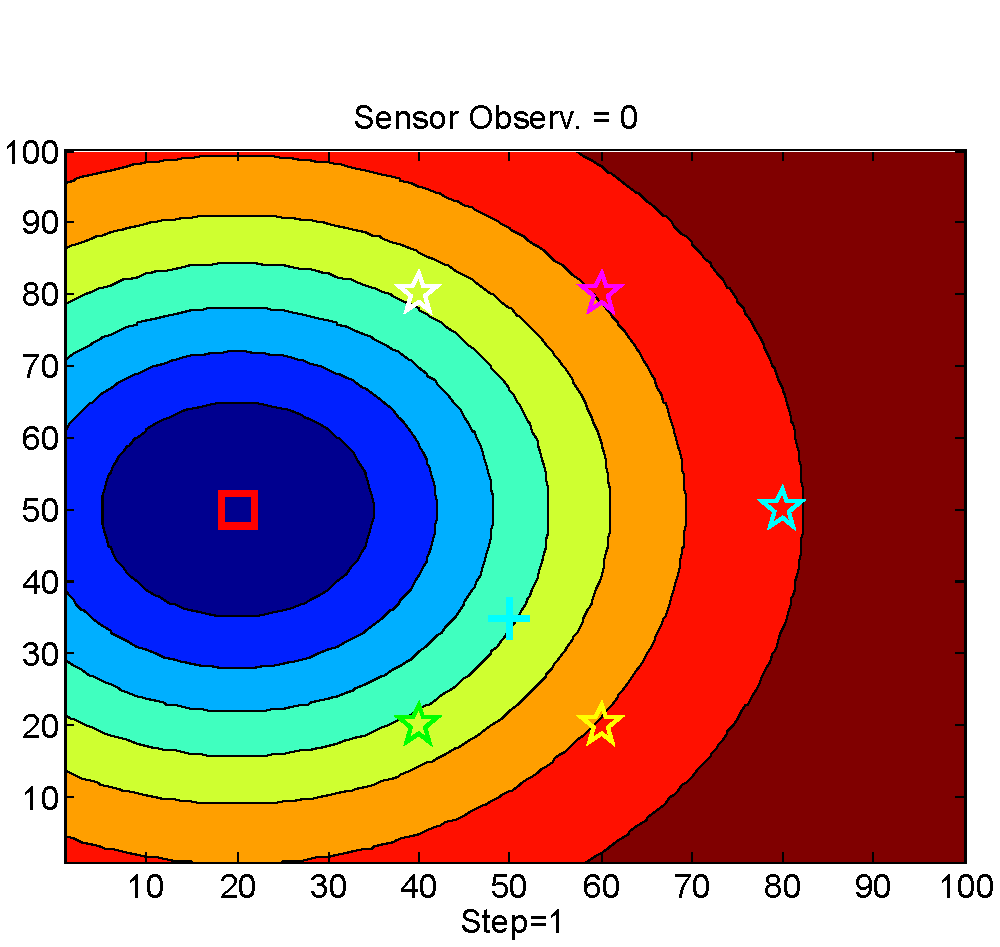
\includegraphics[width=\textwidth]{figures/sta_sen_sta_tar_single_1}
		\caption{Step 1}\label{fig:sta_sen_sta_tar_sing1}
	\end{subfigure}
	\begin{subfigure}[b]{0.22\textwidth}
		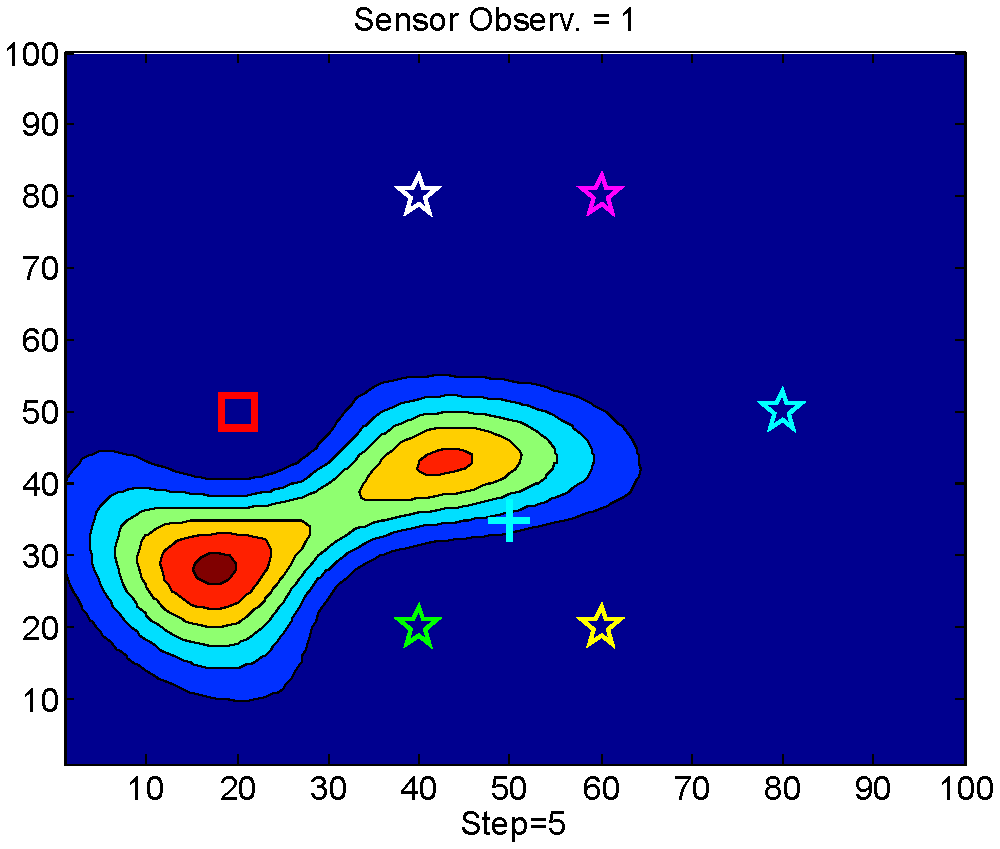
\includegraphics[width=\textwidth]{figures/sta_sen_sta_tar_single_5}
		\caption{Step 5}\label{fig:sta_sen_sta_tar_sing2}
	\end{subfigure}
	\begin{subfigure}[b]{0.22\textwidth}
		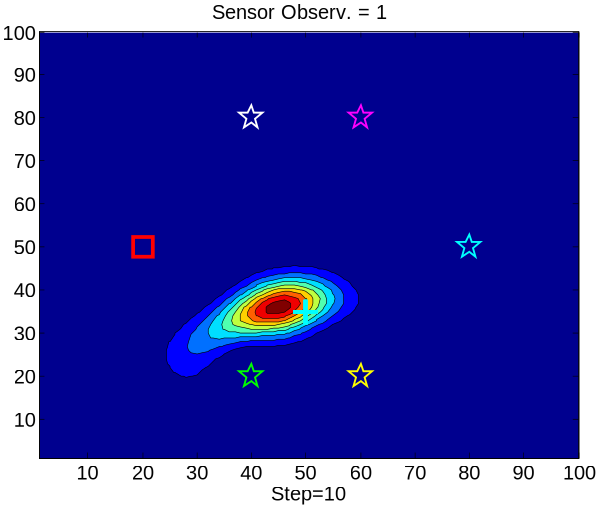
\includegraphics[width=\textwidth]{figures/sta_sen_sta_tar_single_10}
		\caption{Step 10}\label{fig:sta_sen_sta_tar_sing3}
	\end{subfigure}
	\begin{subfigure}[b]{0.22\textwidth}
		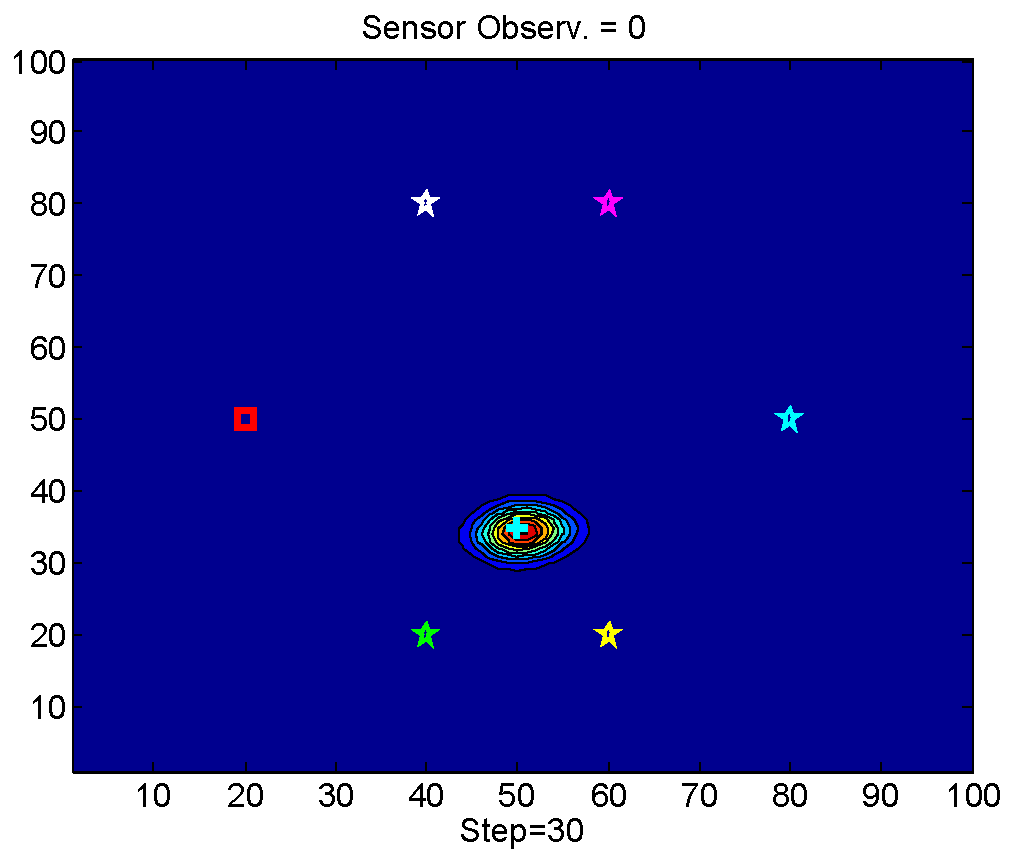
\includegraphics[width=\textwidth]{figures/sta_sen_sta_tar_single_30}
		\caption{Step 30}\label{fig:sta_sen_sta_tar_sing4}
	\end{subfigure}
	\begin{subfigure}[b]{0.48\textwidth}
		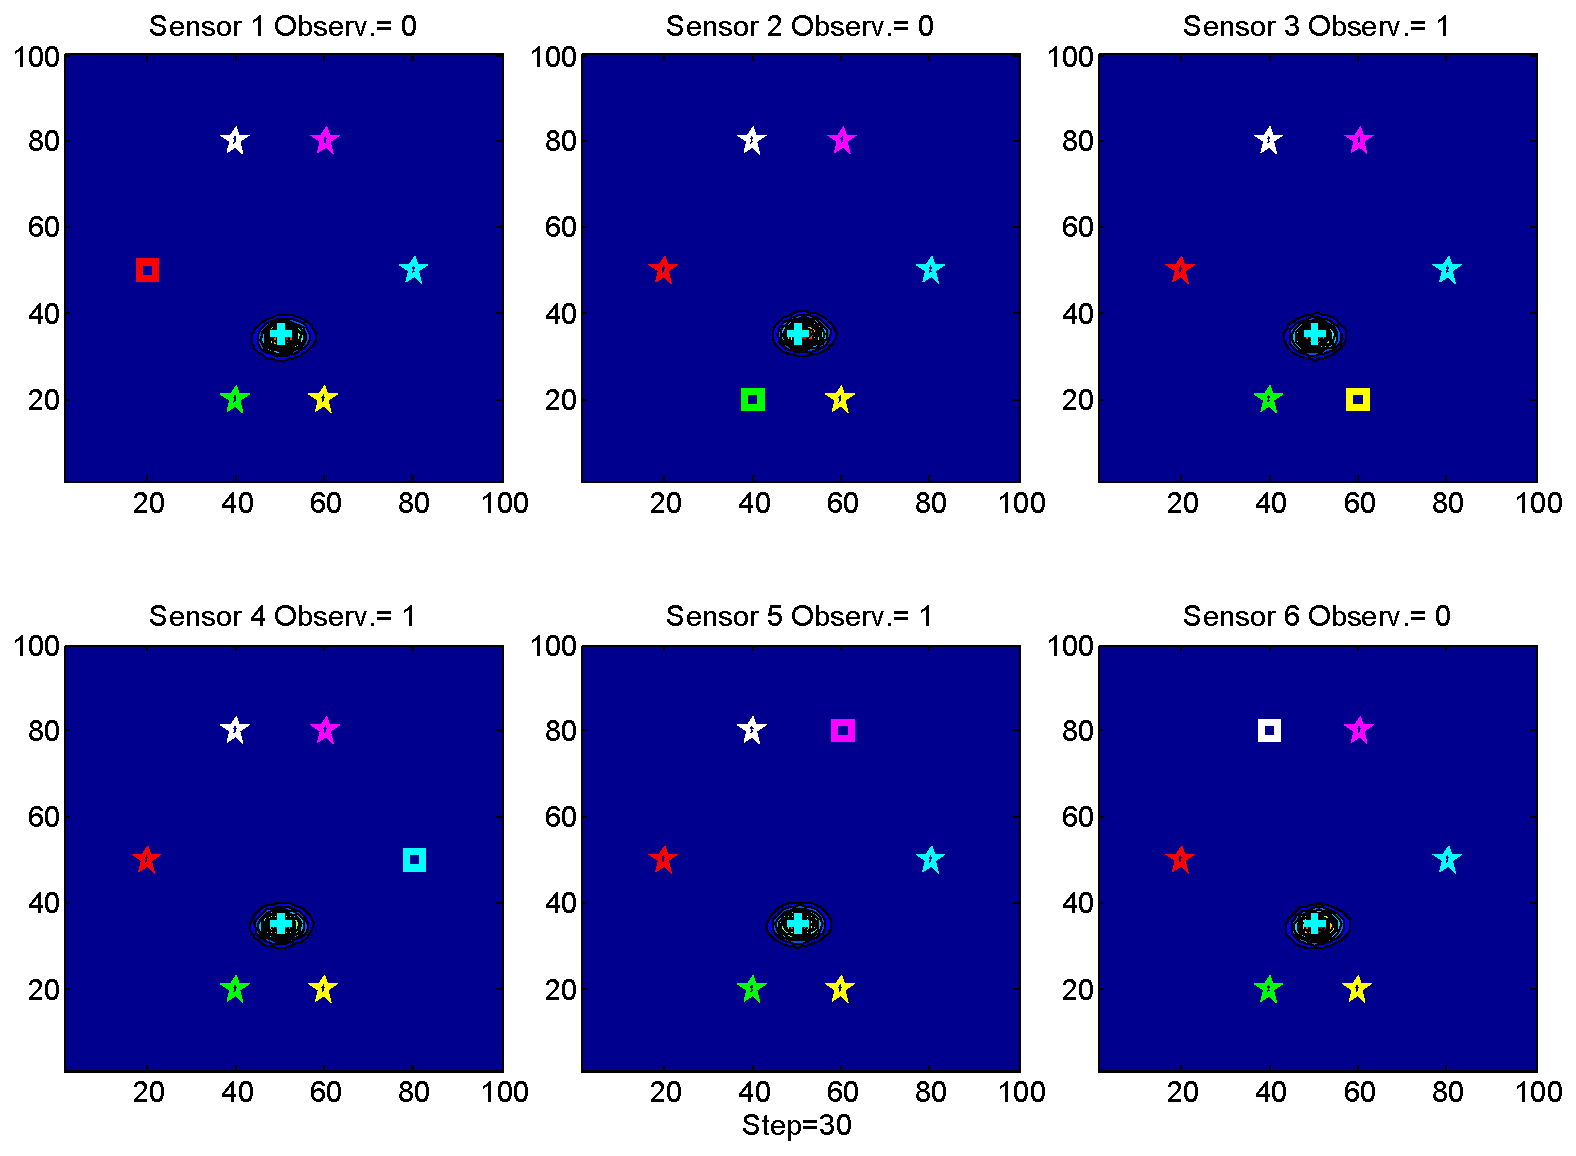
\includegraphics[width=\textwidth]{figures/sta_sen_sta_tar_30}
		\caption{Step 30}\label{fig:sta_sen_sta_tar_all}
	\end{subfigure}
	\caption{(a)-(d): The $1^\text{st}$ robot's individual PDFs at different time; (e) All robots' individual PDFs at time $30$. The square denotes the current robot and stars represent other robots. The cross stands for the target.}
	\label{fig:sta_sen_sta_tar}
\end{figure}

\begin{figure}%[thpb]
	\centering
	\begin{subfigure}[b]{0.22\textwidth}
		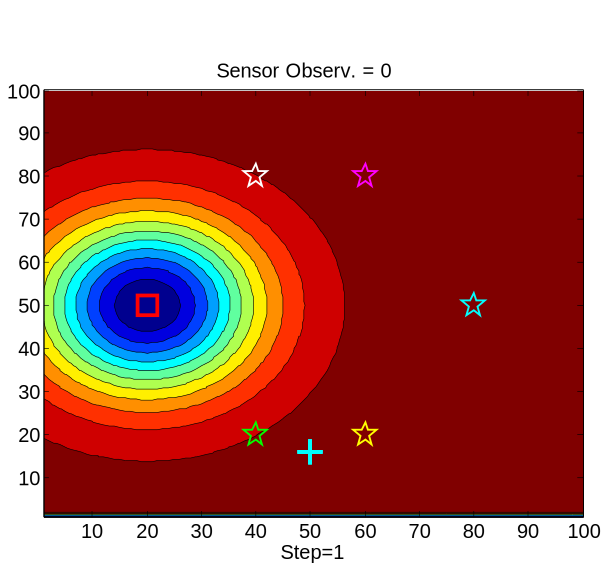
\includegraphics[width=\textwidth]{figures/mov_sen_mov_tar_single_1}
		\caption{Step 1}\label{fig:mov_sen_mov_tar_sing1}
	\end{subfigure}
	\begin{subfigure}[b]{0.22\textwidth}
		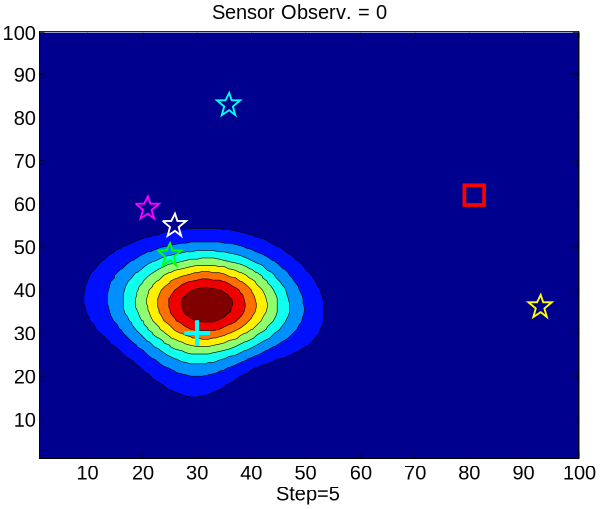
\includegraphics[width=\textwidth]{figures/mov_sen_mov_tar_single_5}
		\caption{Step 5}\label{fig:mov_sen_mov_tar_sing2}
	\end{subfigure}	
	\begin{subfigure}[b]{0.22\textwidth}
		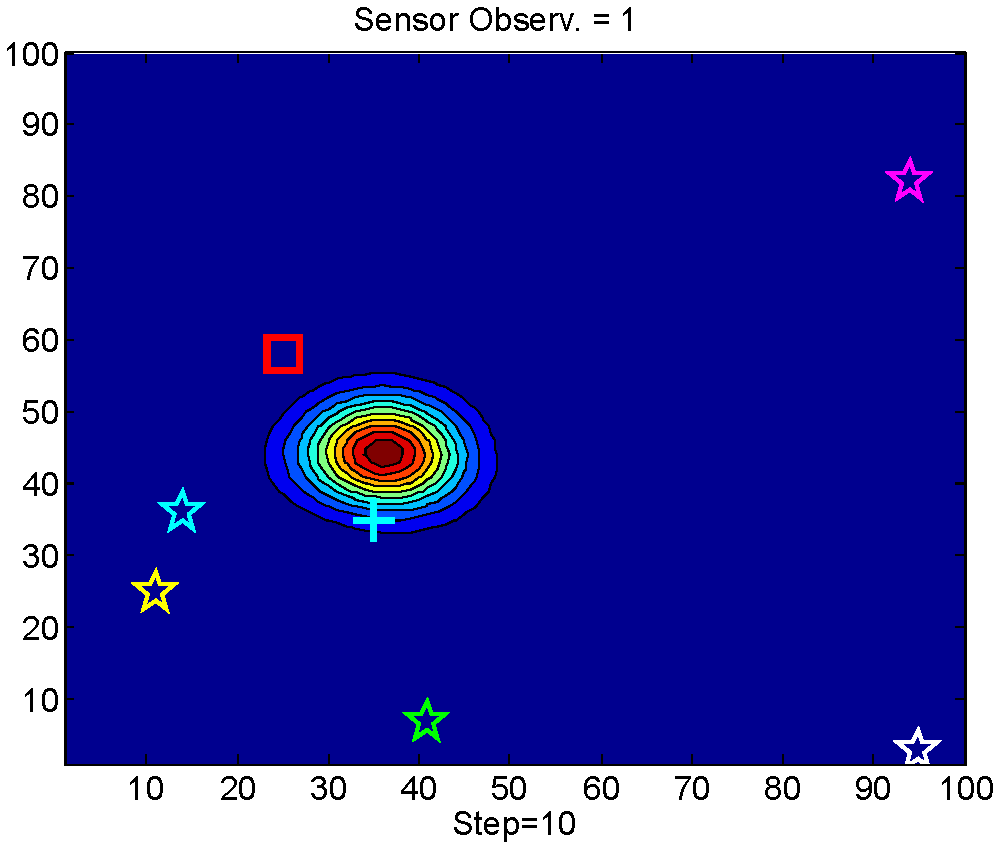
\includegraphics[width=\textwidth]{figures/mov_sen_mov_tar_single_10}
		\caption{Step 10}\label{fig:mov_sen_mov_tar_sing3}
	\end{subfigure}	
	\begin{subfigure}[b]{0.22\textwidth}
		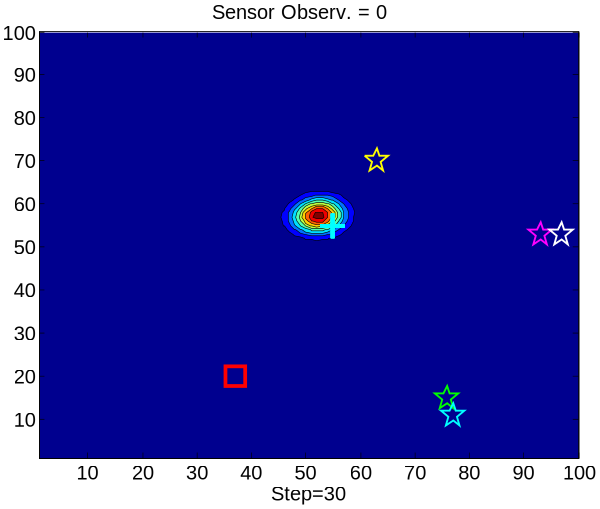
\includegraphics[width=\textwidth]{figures/mov_sen_mov_tar_single_30}
		\caption{Step 30}\label{fig:mov_sen_mov_tar_sing4}
	\end{subfigure}
	\begin{subfigure}[b]{0.48\textwidth}
		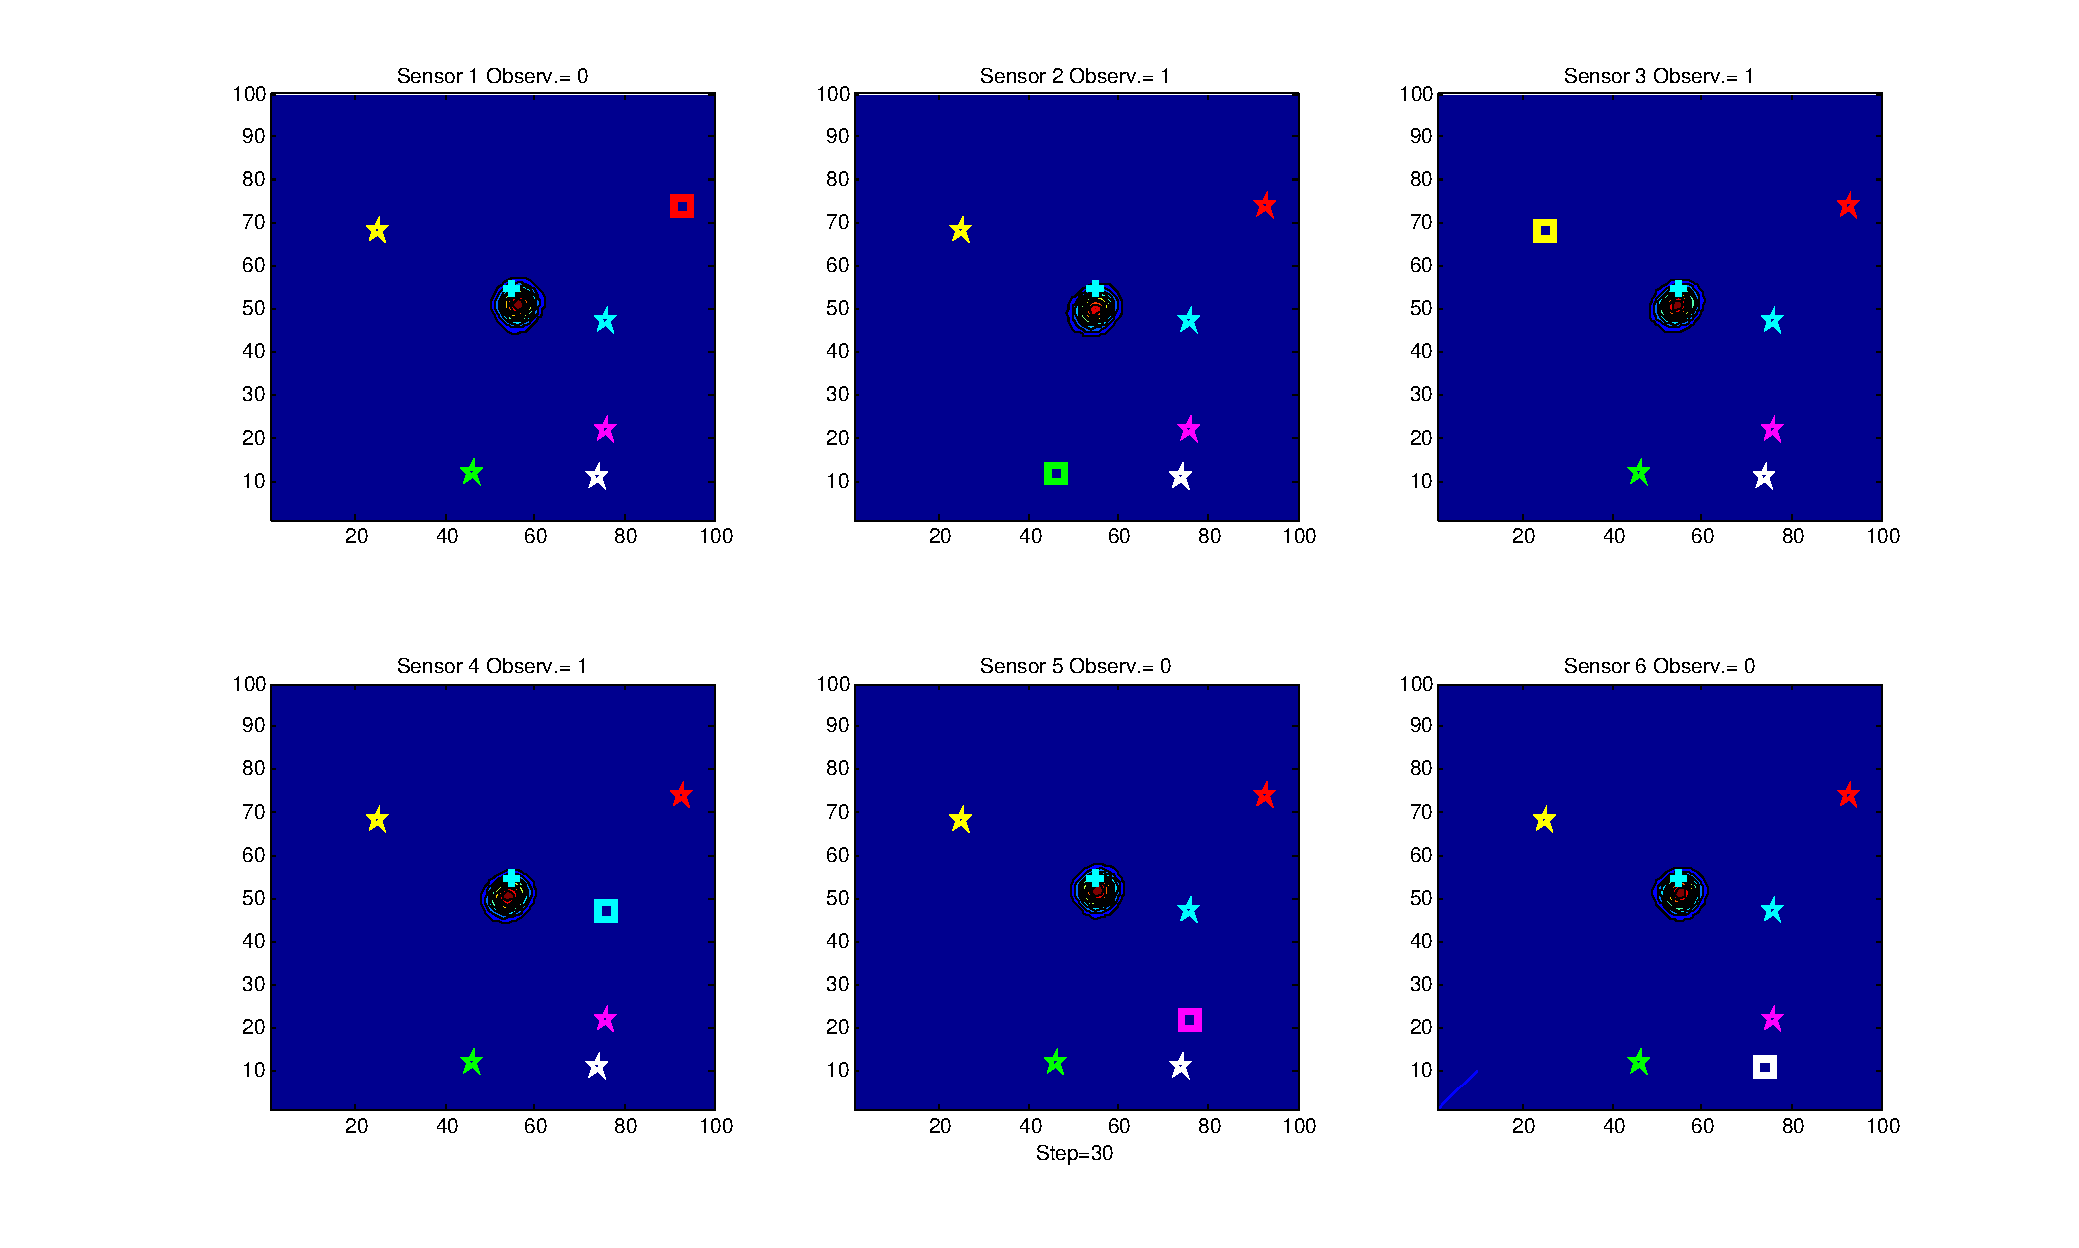
\includegraphics[width=\textwidth]{figures/mov_sen_mov_tar_30}
		\caption{Step 30}\label{fig:mov_sen_mov_tar_all}
	\end{subfigure}
	\caption{(a)-(d): The $1^\text{st}$ robot's individual PDFs at different time; (e) All robots' individual PDFs at time $30$.}
	\label{fig:mov_sen_mov_tar}
\end{figure}

This section simulates three scenarios of target localization to demonstrate the effectiveness of LIFO-BDF. 
In all scenarios, six robots are utilized and each robot is equipped with a binary sensor. 
All sensors are modeled with identical Gaussian functions:
%\small\begin{align}\label{eqn:gauss_sensor}
\small\begin{subequations}\label{eqn:gauss_sensor}
	\begin{align}
		P(z=1|x^T;x^R)&=\exp\left\lbrace -\frac{1}{2}(x^T-x^R)^T{\Sigma}^{-1}(x^T-x^R)\right\rbrace \\
		P(z=0|x^T;x^R)&=1-P(z=1|x^T;x^R).
	\end{align}
\end{subequations}\normalsize
%\end{align}\normalsize
%where $x^s$ denotes the robot position where current observation is obtained. 
%Figure 4 shows the 1-D illustration of Gaussian binary sensor model.
%where $x^R$ denotes the robot position, which is included in robot state $y^R$.

The first scenario consists of six static robots and single static target.
%, which acts as a proof of concept of LIFO-DBF for static target.
The second scenario subsequently deals with six moving robots for localizing a single static target. 
Robot positions are randomly generated at each time step. 
The third scenario contains six moving sensors and one moving target. 
A single-integrator dynamics is used for the target motion model.

\subsection{Static Robots, Static Target}\label{subsec:sim1}

The positions of six static robots are shown as stars in \cref{fig:sta_sen_sta_tar}.
%Each robot constantly receives binary observations of the target.
The LIFO-DBF for static target is implemented on each robot for target position estimation.
\cref{fig:sta_sen_sta_tar} shows the estimation results of the static target. 
After the initial observation, each robot forms a circular individual PDF, centered at its own position.
%\cref{fig:sta_sen_sta_tar_sing1} shows the individual PDF after initial observation for $1^\text{st}$ robot.
The circular PDF happens because the Gaussian sensor model (\Cref{eqn:gauss_sensor}) only depends on the distance between robot and target.
As more observations are received, the posterior individual PDF concentrates \todohere{concentrate or converge?} on the true location of the target (\cref{fig:sta_sen_sta_tar_sing4}), which accords with the consistency of LIFO-DBF.
%In fact, with the Guassian sensor model (\Cref{eqn:gauss_sensor}), all positions with equal distance to a robot belong to the same equi-parameter set of the robot.
%Considering the system of six robots located separately, the equi-parameter set that contains the actual target position only contains one element.
%\cref{fig:entropy} (a) shows the decrease of the entropy of each robot's individual PDF, indicating the reduction of the uncertainty in PDF estimation.

%\subsection{Moving Robots, Static Target}
%The six robots move within the field to estimate the target position. 
%The motion planning of robots for effective target search has received much attention in the past years. 
%In this work, the robot positions are randomly generated at each time in order to demonstrate the effectiveness of LIFO-DBF approach. 
%Readers interested in robot motion planning can refer to \cite{tisdale2009autonomous,furukawa2006recursive}.
%
%\cref{fig:mov_sen_sta_tar} shows the estimation results over time. 
%Similar to the results in \cref{subsec:sim1}, the posterior individual PDF concentrates to the true target location. 
%\cref{fig:entropy} (b) shows the decrease of the entropy of the individual PDFs.
%
%\begin{figure}%[thpb]
%	\centering
%	\begin{subfigure}[b]{0.23\textwidth}
%		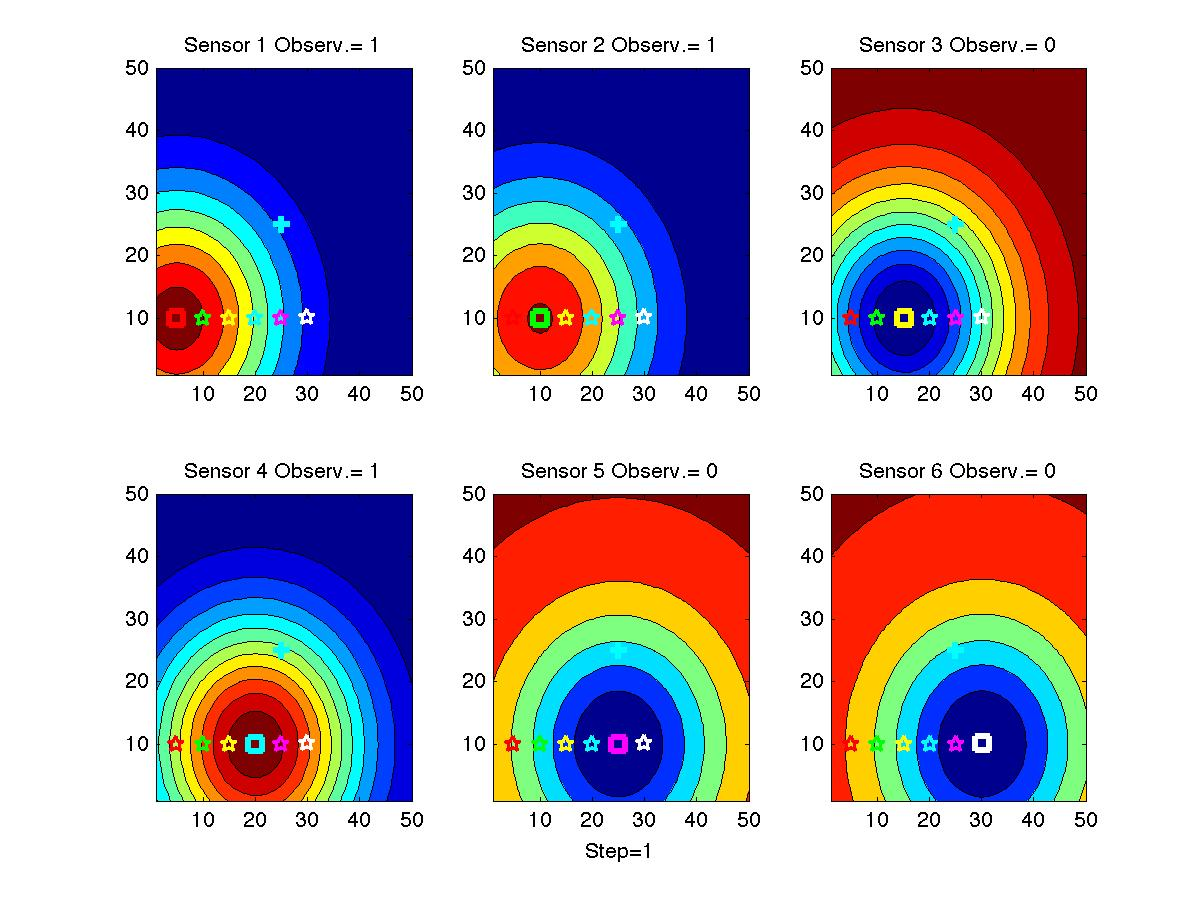
\includegraphics[width=\textwidth]{figures/mov_sen_sta_tar_1}
%		\caption{Step 1}\label{fig:mov_sen_sta_tar1}
%	\end{subfigure}
%	~
%	\begin{subfigure}[b]{0.23\textwidth}
%		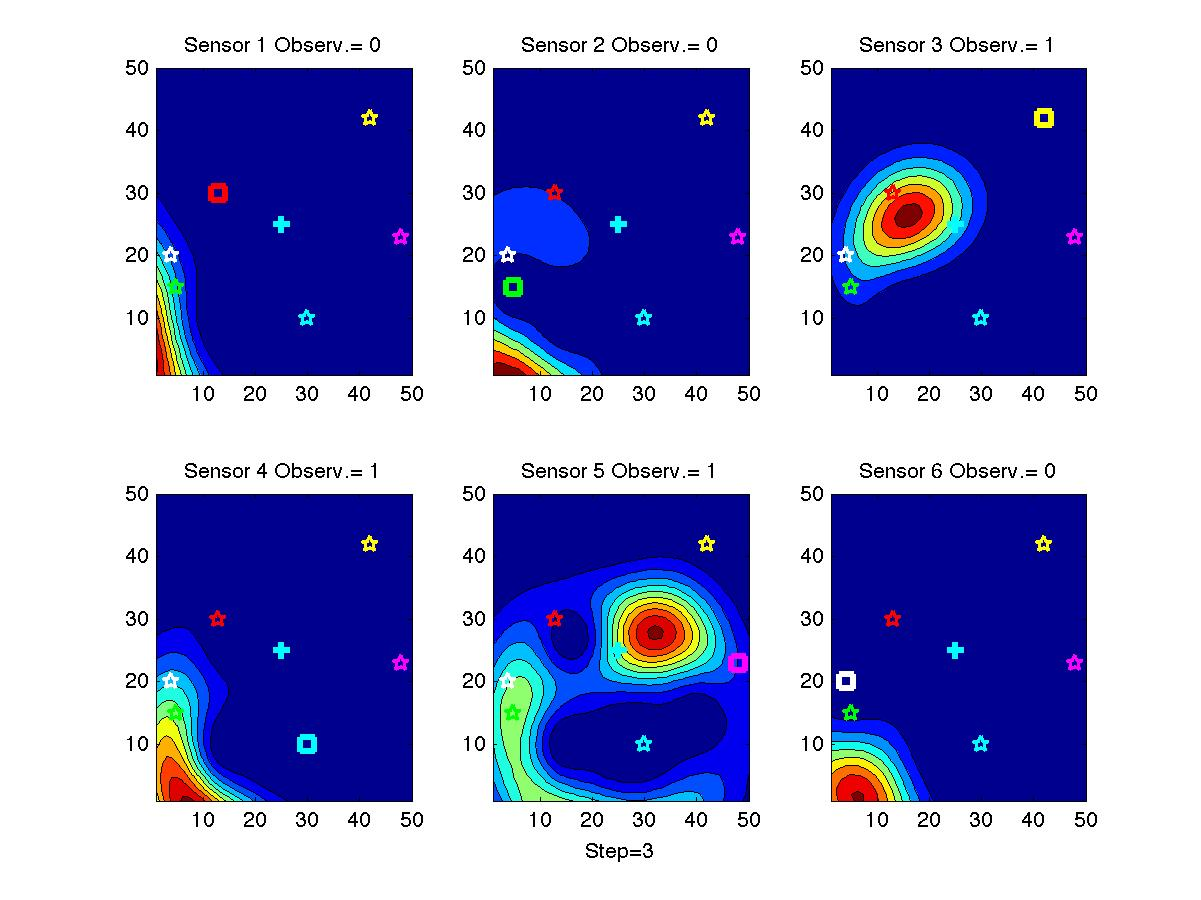
\includegraphics[width=\textwidth]{figures/mov_sen_sta_tar_3}
%		\caption{Step 3}\label{fig:mov_sen_sta_tar2}
%	\end{subfigure}
%	~
%	\begin{subfigure}[b]{0.23\textwidth}
%		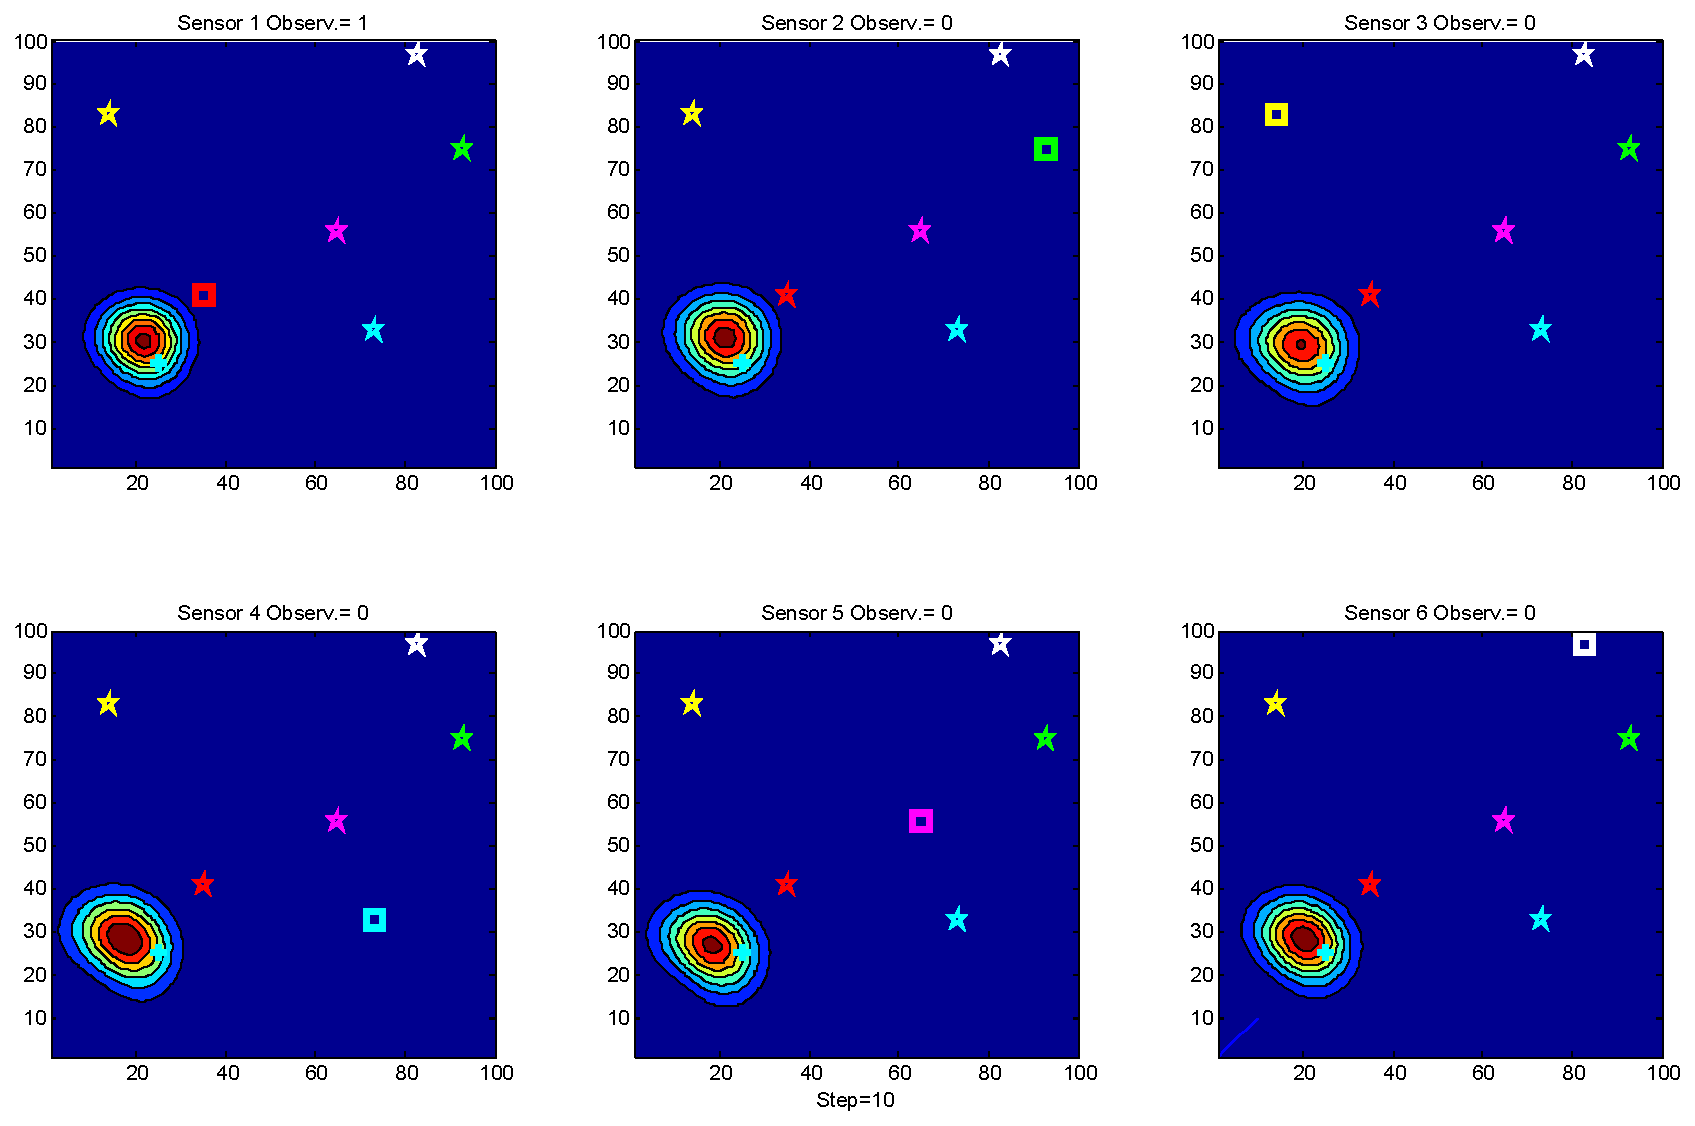
\includegraphics[width=\textwidth]{figures/mov_sen_sta_tar_10}
%		\caption{Step 10}\label{fig:mov_sen_sta_tar3}
%	\end{subfigure}
%	~
%	\begin{subfigure}[b]{0.23\textwidth}
%		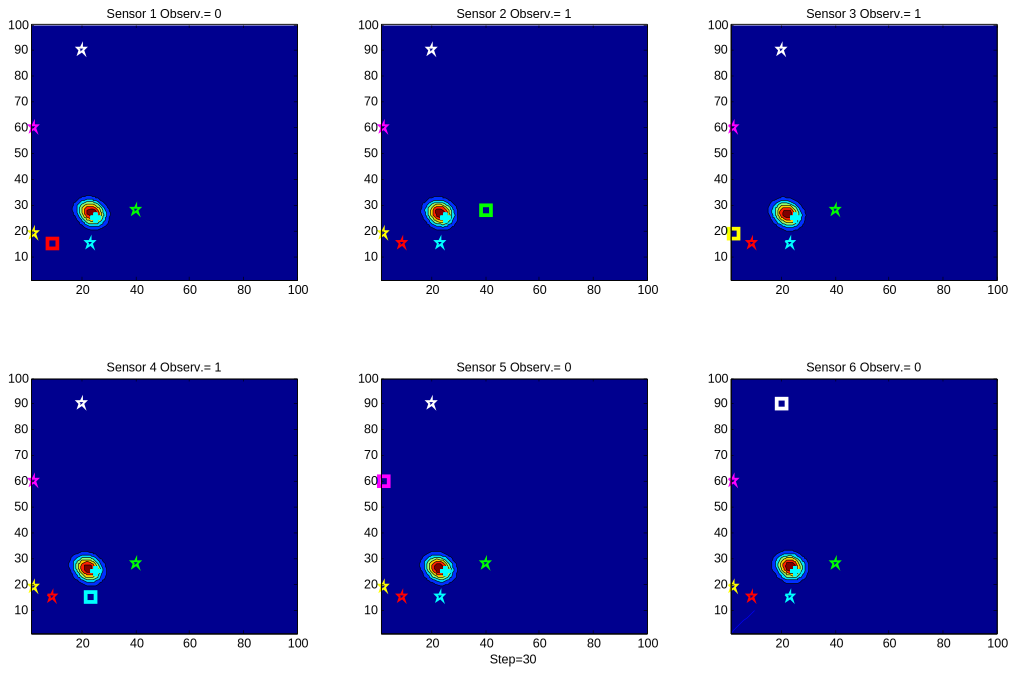
\includegraphics[width=\textwidth]{figures/mov_sen_sta_tar_30}
%		\caption{Step 30}\label{fig:mov_sen_sta_tar4}
%	\end{subfigure}
%	\caption{Moving robots' individual PDFs of the static target.}
%	\label{fig:mov_sen_sta_tar}
%\end{figure}

\subsection{Moving Robots, Moving Target}
The six robots move within the field to estimate the target position. 
%The motion planning of robots for effective target search has received much attention in the past years. 
%Readers interested in this topic can refer to \cite{tisdale2009autonomous,furukawa2006recursive}.
In this work, the robot positions are randomly generated at each time in order to demonstrate the effectiveness of LIFO-DBF approach. 
The target dynamics is given by a single-integrator model:
\begin{equation*}
x^T(k+1)=x^T(k)+v\Delta T
\end{equation*}
where $v$ is the constant velocity of the target; $\Delta T$ is the sampling time.

The LIFO-DBF described in \cref{subsec:LIFO-dbf-mov-tar} is utilized for target localization.
\cref{fig:mov_sen_mov_tar} shows the estimation results of the moving target. 
It is interesting to notice that the posterior individual PDFs concentrate to the true target location at each time, even when the target constantly moves.
%\cref{fig:entropy} (b) shows the decrease of the entropy of the posterior distribution.

%\begin{figure}%[thpb]
%	\centering
%	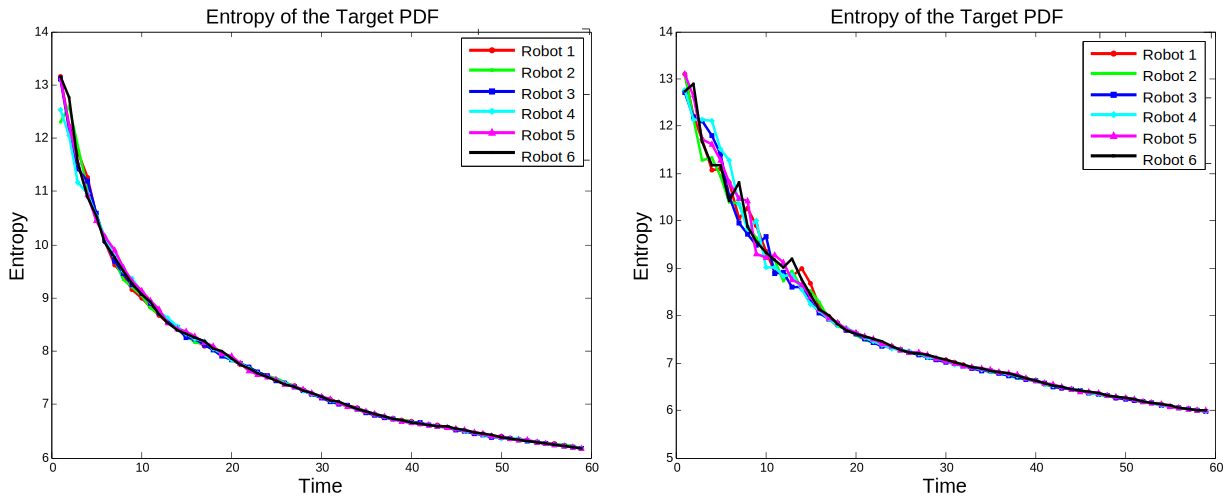
\includegraphics[width=0.5\textwidth]{figures/entropy_all}
%	\caption{Entropy of individual PDFs over time: (a) static robots and static target; (b) moving robots and moving target.}
%	\label{fig:entropy}
%\end{figure}

\section{CONCLUSION}\label{sec:conclu}
This paper presents the Latest-In-and-Full-Out (LIFO) strategy for measurement dissemination-based distributed Bayesian filters (DBF) in a multi-robot network.
% for target search and tracking.
Different from statistics dissemination approaches that transmit posterior distributions or likelihood functions, each robot under LIFO only receives the latest available measurements and then broadcasts full communication buffer to its neighborhood, which significantly reduces the transmission burden of each pair from the order of environmental size to that of robot number.
Under the condition of fixed and undirected topology, LIFO can guarantee non-intermittent dissemination of all observations over the network within finite time via local communication among neighbors.
%, with each robot non-intermittently receiving observations of all others.
Two types of LIFO-based DBF algorithms are proposed to estimate individual PDF for static and moving target, respectively. 
For the static target, each robot locally fuses the newly received observations while for the moving target, a triangular matrix of historical observations is stored and updated. 
%Upon obtaining the latest available observations of all robots, an iterative Bayesian filtering procedure is applied that alternates between prediction and updating steps. 
The consistency of LIFO-based DBF is proved utilizing law of large numbers, which ensures that individual PDF of each robot converges to the true target position when the number of observations tends to infinity.
%the agreement between robots' estimated target position and the actual position.
%The effectiveness of this method is demonstrated by simulations.
\todohere{find out what convergence is}

%In this study, we proposed the Latest-In-and-Full-Out (LIFO) strategy for distributed Bayesian filters (LIFO-DBF) in a multi-robot network.
%% with the application of distributed search and tracking (SAT) of target.
%With fixed communication topology, LIFO guarantees the global dissemination of all robots' observations over the network only via local exchange of observations among neighbors.
%Once elements in communication buffer (CB) gets filled, each robot can receive and update its CB non-intermittently under LIFO.
%Two LIFO-DBFs are proposed for SAT of a static and a moving target, respectively. 
%For the static target, each robot locally fuses the latest knowledge of all robots' observations by only considering the updating step of the Bayesian filter. 
%For the moving target, each robot maintains a triangle matrix of historical observations and an iterative Bayesian filtering procedure is applied that alternates between prediction and updating steps upon obtaining the latest available observations of all robots. 
%The consistency of LIFO-DBF is proved by showing the asymptotic concentration of posterior individual PDF to the equi-parameter set containing the actual state, ensuring the agreement between robots' state estimate using LIFO-DBF and the actual environment state.
%Simulations demonstrate the effectiveness of LIFO-DBF for SAT of both static and moving targets.

Future work includes extensions to other types of sensors and switching topology.
Other types of sensors may have biased observations and subject to non-Bernoulli distribution, which complicates the design and analysis of LIFO-based Bayesian filters.
The switching topology, including package loss, can lead to unpredictable delay and intermittent transmission, which may affect the consistency and consensus of individual PDFs. 
%In addition, combining LIFO-DBF with robot motion planning is promising for more effective SAT of target.


\addtolength{\textheight}{-12cm}   % This command serves to balance the column lengths
                                  % on the last page of the document manually. It shortens
                                  % the textheight of the last page by a suitable amount.
                                  % This command does not take effect until the next page
                                  % so it should come on the page before the last. Make
                                  % sure that you do not shorten the textheight too much.

%%%%%%%%%%%%%%%%%%%%%%%%%%%%%%%%%%%%%%%%%%%%%%%%%%%%%%%%%%%%%%%%%%%%%%%%%%%%%%%%



%%%%%%%%%%%%%%%%%%%%%%%%%%%%%%%%%%%%%%%%%%%%%%%%%%%%%%%%%%%%%%%%%%%%%%%%%%%%%%%%



%%%%%%%%%%%%%%%%%%%%%%%%%%%%%%%%%%%%%%%%%%%%%%%%%%%%%%%%%%%%%%%%%%%%%%%%%%%%%%%%
%\section*{APPENDIX}
%
%Appendixes should appear before the acknowledgment.

%\section*{ACKNOWLEDGMENT}
%
%The preferred spelling of the word �acknowledgment� in America is without an �e� after the �g�. Avoid the stilted expression, �One of us (R. B. G.) thanks . . .�  Instead, try �R. B. G. thanks�. Put sponsor acknowledgments in the unnumbered footnote on the first page.



%%%%%%%%%%%%%%%%%%%%%%%%%%%%%%%%%%%%%%%%%%%%%%%%%%%%%%%%%%%%%%%%%%%%%%%%%%%%%%%%
\bibliographystyle{IEEEtran}
%\bibliographystyle{bibtex}
\bibliography{references}

\end{document}
